\documentclass[11pt]{article}
\usepackage[margin=1in]{geometry}
\usepackage{amsmath,amssymb,graphicx,hyperref,xurl,parskip,booktabs,longtable}
\usepackage[T1]{fontenc}
\usepackage[utf8]{inputenc}
\usepackage{caption}
\hbadness=10000
\hfuzz=20pt
\setlength{\emergencystretch}{3em}
\hypersetup{colorlinks=true,linkcolor=black,citecolor=black,urlcolor=blue}
\title{From Discourse to Structure: A Knowledge Graph-Based Approach to Topic Modeling in Political Debate}
\author{}
\date{}
\begin{document}
\maketitle

\begin{abstract}
Can we extract meaningful political topics from parliamentary speeches by building a knowledge graph and detecting communities within it? This thesis explores that question. Rather than treating topic modeling as a bag-of-words problem in the tradition of Latent Dirichlet Allocation (LDA), the approach taken here constructs an explicit knowledge graph from text---using ontology-guided, large language model (LLM) extraction---and then identifies topics as densely connected communities of entities and relationships within that graph.

The methodology is applied to the verbatim reports of the `This is Europe' European Parliamentary debate series (2022--2024), a corpus of 13 speeches by EU Heads of State or Government. These debates took place during an unprecedented confluence of crises---Russia's invasion of Ukraine, the energy crisis, migration pressures---making the corpus both thematically rich and highly interconnected. An independent expert analysis by the European Parliamentary Research Service (EPRS) serves as the ground truth against which the pipeline's output is evaluated.

The pipeline proceeds in measurable stages. First, unstructured text is transformed into a knowledge graph using a ``just-enough-semantics'' design: each text chunk is semantically matched to a domain ontology (the EU's Common Data Model family) that constrains which \emph{types} of entities the LLM may extract, while the relationships between those entities emerge freely from the text. The resulting graph (7{,}975 nodes, 4{,}841 resolved entities) exhibits a heavy-tailed, scale-free degree distribution (Clauset maximum-likelihood exponent $\alpha \approx 2.38$, KS distance $0.023$), consistent with organically grown networks. Second, node2vec embeddings reweight the graph's edges by topological similarity before the Leiden community detection algorithm partitions it into topics. This reweighting lifts the modularity score from a baseline of $0.702$ to $0.812$---an absolute gain of $+0.110$ ($+15.7\%$)---an improvement that a permutation test ($p<0.001$) and a 20-seed stability analysis (Cohen's $d = 58.9$) confirm is large and reproducible. Third, the detected communities are summarised by a 70-billion-parameter LLM into structured analytical reports. The resulting 99 communities range from a dominant ``European Union Community Dynamics'' cluster (716 entities) to niche national debates such as ``Erosion of Democratic Norms in Slovenia'' (5 entities) and ``Missing Cypriots: Unresolved Disappearances'' (3 entities).

When compared to the EPRS ground truth, the pipeline's topics align well: all six of the EPRS's recurring themes are recovered (100\% coverage, mean best-match similarity $0.444$), with the largest communities capturing the dominant themes (Ukraine, energy, EU unity) and the smallest isolating the national policy debates that the EPRS records as secondary. Benchmarked against a classical Latent Dirichlet Allocation (LDA) model trained on the identical corpus and scored on the same metric, the graph pipeline is both more complete (LDA recovers only 5 of 6 themes at matched granularity) and more precisely aligned (mean similarity $0.444$ vs.\ LDA's $0.351$). The subtopic similarity distribution is unimodal and centred near $\mu \approx 0.47$, reflecting a corpus that is unified in subject but genuinely differentiated in sub-themes. A persistently negative entity silhouette ($-0.26$ at the community level) shows that these communities are \emph{structurally} rather than \emph{semantically} separated---an honest signature of a discourse in which every leader speaks about the same crises in overlapping language. These results suggest that graph-based community detection offers a promising direction for topic modeling in political discourse, particularly in corpora where standard probabilistic methods struggle with thematic overlap.
\end{abstract}

\hrule

\section{Chapter 1: From `Topic' to Graph Community}

\subsection{1.1 What Is a Topic, and Why Does It Matter?}

The word ``topic'' is used loosely in data science. In practice it usually means ``a cluster of words that tend to co-occur.'' But the concept has deeper roots. In linguistics, the foundational distinction is between the \emph{topic} (what a clause is about) and the \emph{comment} (what is being said about it)---what Halliday (1985) called the \emph{theme--rheme} structure of information. A topic, in this sense, is not a bag of words but an anchor: the entity or concept that organises the surrounding propositions.

The philosophy of language adds another layer through the notion of ``aboutness'' (Reinhart, 1981). A topic is the thing the speaker directs the hearer's attention to, the subject about which information is conveyed. This is a pragmatic definition, grounded in communicative intent rather than syntactic position. It sets a higher bar for computational topic modeling: the goal should not merely be to find co-occurring terms, but to identify the primary subjects of ``aboutness'' that structure a body of text.

This relational view of topics---where a topic is defined not in isolation but by its connections to other concepts---resonates with Foucault's (1972) characterisation of discourse as a ``system of thoughts'' in which meaning arises from the interplay of statements. If topics are constituted by relationships, then a representation that makes those relationships explicit should, in principle, capture them better than one that discards relational structure entirely.

\subsection{1.2 From Probabilistic to Structural Topic Modeling}

The dominant computational approach to topic modeling for the past two decades has been the probabilistic paradigm, exemplified by Latent Dirichlet Allocation (LDA) (Blei, Ng, \& Jordan, 2003). LDA defines a topic as a probability distribution over a vocabulary, inferred from word co-occurrence patterns within documents. This relies on the ``bag-of-words'' assumption, which treats text as an unordered collection of terms and discards syntax, reference, and relational structure.

This thesis takes a different approach: a \emph{structural} one. Instead of inferring latent word distributions, it constructs an explicit knowledge graph from the text and identifies topics as communities within that graph. The working definition is straightforward:

\emph{A topic is a densely interconnected community of entities (nodes) and their relationships (edges) within a knowledge graph, identified through community detection and articulated through a natural language summary.}

This is not an isolated intuition. There is a growing body of work treating topics as network communities rather than latent word distributions. Gerlach, Peixoto \& Altmann (2018) show that representing a corpus as a bipartite document--word network and applying a hierarchical stochastic block model is a principled generalisation of topic modeling---LDA is recoverable as a restricted parametrisation of the block model---and argue that the network formulation better matches the statistical properties of real text while automatically inferring the number of topics. Working directly on word graphs, Chowdhury et al.\ (2023) formulate topic modeling as community detection on a word-association network and report results competitive with, and in most of their test cases superior to, established probabilistic topic models. The present work extends this community-as-topic logic from co-occurrence graphs of \emph{words} to an LLM-extracted knowledge graph of \emph{entities and relations}, and---unlike those studies---evaluates the result against an independent expert analysis of the same corpus.

This moves the unit of analysis from words to entities---people, organisations, places, policies---and their explicit, labelled relationships. The question this thesis asks is whether such communities, when detected algorithmically and summarised by an LLM, correspond to the topics that a human expert would identify in the same corpus. The answer, as the following chapters will show, is encouraging but nuanced.

\hrule

\section{Chapter 2: Building a Knowledge Graph from Parliamentary Debate}

\subsection{2.1 The Corpus and Its Ground Truth}

The corpus consists of the verbatim reports of the `This is Europe' debate series held in the European Parliament between April 2022 and March 2024. In this series, 13 EU Heads of State or Government addressed the Parliament to present their visions for the future of the European Union.

The timing matters. The debates commenced shortly after Russia's full-scale invasion of Ukraine, a geopolitical event that reshaped European priorities overnight. They also ran concurrently with the conclusion of the Conference on the Future of Europe (CoFoE), a citizen-led initiative to guide EU policy. This backdrop means that while each leader brought a distinct national perspective, the speeches were anchored in a shared set of urgent challenges.

An independent analysis of these debates by Drachenberg \& B\k{a}cal for the European Parliamentary Research Service (EPRS, 2024) provides a detailed ground truth. The EPRS identifies 43 specific topics addressed by the speakers, grouped into seven macro-categories: (i) policies, (ii) crises, (iii) European integration, (iv) national topics, (v) democracy, (vi) external relations, and (vii) geopolitical Europe. Their quantitative findings include:

\begin{itemize}
  \item \textbf{Ukraine} was mentioned by all 13 speakers and received 14\% of total speech attention---the dominant topic by both breadth and depth.
  \item \textbf{Energy} was the second-most discussed policy area, accounting for 26\% of all policy-related attention, followed by \textbf{enlargement} at 24\%.
  \item \textbf{National policies}---specific to individual Member States---accounted for 7\% of attention and were driven primarily by the speeches of Mitsotakis (Greece) and Christodoulides (Cyprus).
  \item Six recurring themes appeared across speakers: the value of EU membership, defending EU values, the EU's main challenges, delivering for citizens, next steps in integration, and EU unity.
\end{itemize}

This corpus is a stringent test for any topic model. The high degree of thematic overlap and shared vocabulary makes it difficult for purely statistical methods to disentangle sub-topics---when every speaker discusses Ukraine, energy, and EU unity, word co-occurrence patterns blur together. The EPRS analysis serves as the benchmark against which the graph-based pipeline is evaluated in Chapter 4.

\subsection{2.2 From Text to Graph: The Extraction Pipeline}

The transformation of unstructured text into a structured knowledge graph proceeds through five stages, each governed by a specific design choice. The overarching principle is what I call ``just-enough-semantics'': the pipeline injects the minimum constraint necessary for consistency, while leaving the extraction free enough to surface the organic structure of the discourse.

\paragraph{Stage 1: Ontology Registry and Per-Chunk Matching.}
Before any text is processed, the pipeline loads a registry of domain ontologies and embeds each one. The principal ontology is the EU's Common Data Model (CDM) family, version 4.13.2---the metadata vocabulary that the EU's Publications Office uses to catalogue legal and institutional documents---alongside several related vocabularies (the ECCF core ontology, an organisation ontology, SKOS, and others). For each ontology, the pipeline parses its RDF class files and extracts a title, a natural-language description, and a set of entity-type labels (e.g., \emph{Person}, \emph{Organisation}, \emph{GeopoliticalEntity}, \emph{Policy}, \emph{Event}), retaining only top-level classes with at least one subclass. Each ontology's title, description, and labels are embedded with a sentence-transformer and held in memory.

The key design move is that ontology selection is \emph{per chunk}. When a text chunk is processed, it is embedded and matched by cosine similarity against every ontology description in the registry; the best-matching ontology supplies the entity-type vocabulary for that chunk. In the reported run, nine ontologies were embedded and the extraction drew on a working vocabulary of 29 entity-type labels. This is the ``just-enough'' part: the ontology tells the extraction \emph{what kinds of things} to look for, adapting the vocabulary to each passage, but it does not prescribe \emph{which} specific entities will appear or \emph{how} they will be connected. Entity types are constrained; relationships are free.

\paragraph{Stage 2: Text Chunking.}
The raw verbatim transcripts are segmented into chunks of 512 tokens with a 64-token overlap between consecutive chunks. The chunk size is a design trade-off: smaller chunks yield higher extraction density (more entity mentions per chunk), but at the cost of more LLM calls and the risk of fragmenting multi-sentence arguments. The overlap ensures that relationships spanning a chunk boundary are not lost entirely. The corpus segments into 2{,}085 chunks.

\paragraph{Stage 3: Ontology-Guided Triplet Extraction.}
Each chunk is extracted by a large language model (Llama-3.3-70B-Instruct, accessed through the OpenRouter gateway at temperature 0.0 for determinism), orchestrated with the DSPy framework. The extraction is expressed as a typed DSPy signature: its inputs are the chunk text, the matched ontology's description, and that ontology's list of permitted entity-type labels; its output is a list of \emph{knowledge triplets}, each a Pydantic-validated object carrying a source entity and type, a relation, a target entity and type, a confidence score, and a short span of supporting evidence from the text. Crucially, the entity \emph{types} are drawn from the matched ontology, while the relation labels are \emph{not} constrained---they emerge freely from the text. This asymmetry is the heart of the design: entity types are standardised to prevent hallucination of arbitrary categories, while the relational structure of the graph is left entirely emergent. Using an LLM to extract entities and relations into a usable knowledge graph is by now an established construction---it is the same mechanism GraphRAG employs (Edge et al., 2024), and constraining the extraction with an ontology has been shown to improve the consistency and schema-conformance of the resulting graph (Feng, Wu \& Meng, 2024). It should be stressed, however, that this thesis does not independently benchmark extraction accuracy; the graph is validated downstream, through its network properties (\S2.3) and the correspondence of its communities to the expert ground truth (\S4.3), rather than by a per-triplet gold standard. Extraction succeeded on 2{,}085 of 2{,}085 chunks (4 transient errors, all retried).

\paragraph{Stage 4: Graph Cleaning.}
Raw LLM output is inconsistent. The same real-world entity may appear under different surface forms (``Olaf Scholz,'' ``the German Chancellor,'' ``Mr.\ Scholz''). Entity resolution addresses this in three stages: acronym matching, containment matching, and semantic matching, the last of which embeds all entities with a sentence-transformer model (all-MiniLM-L6-v2) and merges pairs whose cosine similarity exceeds 0.95, subject to a safety check that blocks clearly contradictory merges. On the reported corpus this reduced 5{,}321 raw entities to 4{,}841 (11 acronym, 46 containment, and 423 semantic merges). In addition, edges with extraction confidence below 0.01 are pruned, and isolated nodes are removed.

\paragraph{Stage 5: Graph Assembly.}
The extracted and cleaned elements from all chunks are aggregated into a single, unified knowledge graph. Entities become nodes, relationships become edges, and factual claims extracted alongside the triplets are stored as node attributes. The assembled graph contains \textbf{7{,}975 nodes and 25{,}655 edges} and forms the structured, machine-readable representation of the entire corpus.

\subsection{2.3 A Sanity Check: Does the Graph Behave Like a Real Network?}

If the extraction pipeline has been calibrated correctly---constraining enough to prevent noise, but not so much as to impose artificial structure---the resulting graph should resemble the kind of network that arises organically in the real world. Scale-free networks, characterised by a power-law degree distribution $P(k) \sim k^{-\alpha}$, are ubiquitous in complex systems: the World Wide Web, social networks, citation networks, and biological interaction networks all exhibit this topology (Barab\'{a}si \& Albert, 1999).

The mechanism behind scale-free networks is well understood: \emph{growth} (the network expands over time) combined with \emph{preferential attachment} (new nodes are more likely to connect to already highly connected nodes). Parliamentary debate is consistent with exactly this dynamic. Each speech adds new concepts to the network (growth), and to be relevant, speakers must connect their arguments to the most salient themes already under discussion---Ukraine, energy dependency, EU values---the established hubs (preferential attachment). There is direct precedent for expecting this topology in language data: Ferrer i Cancho \& Sol\'{e} (2001) showed that a word co-occurrence network built from the British National Corpus has a heavy-tailed, approximately power-law degree distribution, and interpreted the word-frequency effect that drives it as a form of preferential attachment. The knowledge graph studied here is a network of \emph{entities} rather than words, but the generative logic is the same.

To test this rigorously, the degree distribution is fitted with the maximum-likelihood method of Clauset, Shalizi \& Newman (2009), rather than by fitting a straight line to a log--log histogram (a procedure those authors specifically caution against, because binning and least-squares fitting on logarithmic axes bias the exponent and cannot distinguish a power law from other heavy-tailed forms). The method estimates the exponent $\alpha$ and the lower cutoff $k_{\min}$ by maximum likelihood, quantifies absolute goodness of fit with the Kolmogorov--Smirnov (KS) distance, and runs likelihood-ratio tests against competing distributions.

The fit yields an exponent $\alpha \approx 2.38$ ($\sigma = 0.08$) above a lower bound $k_{\min}=16$, with a KS distance of $0.023$ and a log--log $R^2 = 0.975$. The exponent sits squarely in the 2--3 range typical of real-world scale-free networks. The likelihood-ratio tests (Table~\ref{tab:lrt}) decisively reject a pure exponential tail in favour of the power law, but---as is almost universal for empirical networks of this size---cannot separate the power law from a log-normal or a truncated power law. The honest conclusion is therefore that the degree distribution is \emph{heavy-tailed and power-law-consistent}.

This caution is deliberate, because the scale-free label is contested in the network-science literature. Broido \& Clauset (2019), applying exactly this maximum-likelihood-plus-likelihood-ratio protocol to nearly a thousand real-world networks, found that strong evidence for a pure power law is the exception rather than the rule, and that heavy tails are often equally well described by a log-normal. The rebuttal by Voitalov et al.\ (2019) argues the opposite conclusion follows if ``scale-free'' is defined more permissively (as a regularly varying tail), which is precisely the definitional looseness this thesis avoids by reporting the KS distance and the likelihood-ratio comparisons openly rather than asserting a pure power law from a visual slope. For the argument here, the strong claim is unnecessary: what matters is that the graph is heavy-tailed with a hub structure in the empirically typical range, not that it is a pristine power law. Had the ontology been too rigid, the graph would instead have shown a uniform, lattice-like structure; had the LLM been under-constrained, it would have approximated a Poisson random graph. The observed heavy tail indicates the extraction struck a reasonable balance and preserved genuine discourse structure.

\begin{table}[h]
\centering
\small
\caption{Likelihood-ratio tests of the power law against alternative distributions. A positive statistic $R$ with $p<0.05$ favours the power law; $p>0.05$ means the two models are statistically indistinguishable on this data.}
\label{tab:lrt}
\begin{tabular}{lccc}
\toprule
\textbf{Alternative} & \textbf{LR statistic $R$} & \textbf{$p$-value} & \textbf{Verdict} \\
\midrule
Exponential         & $+3.86$ & $0.0001$ & Power law strongly favoured \\
Log-normal          & $-1.00$ & $0.32$   & Indistinguishable \\
Truncated power law & $-0.19$ & $0.93$   & Indistinguishable \\
\bottomrule
\end{tabular}
\end{table}

\begin{figure}[h]
\centering
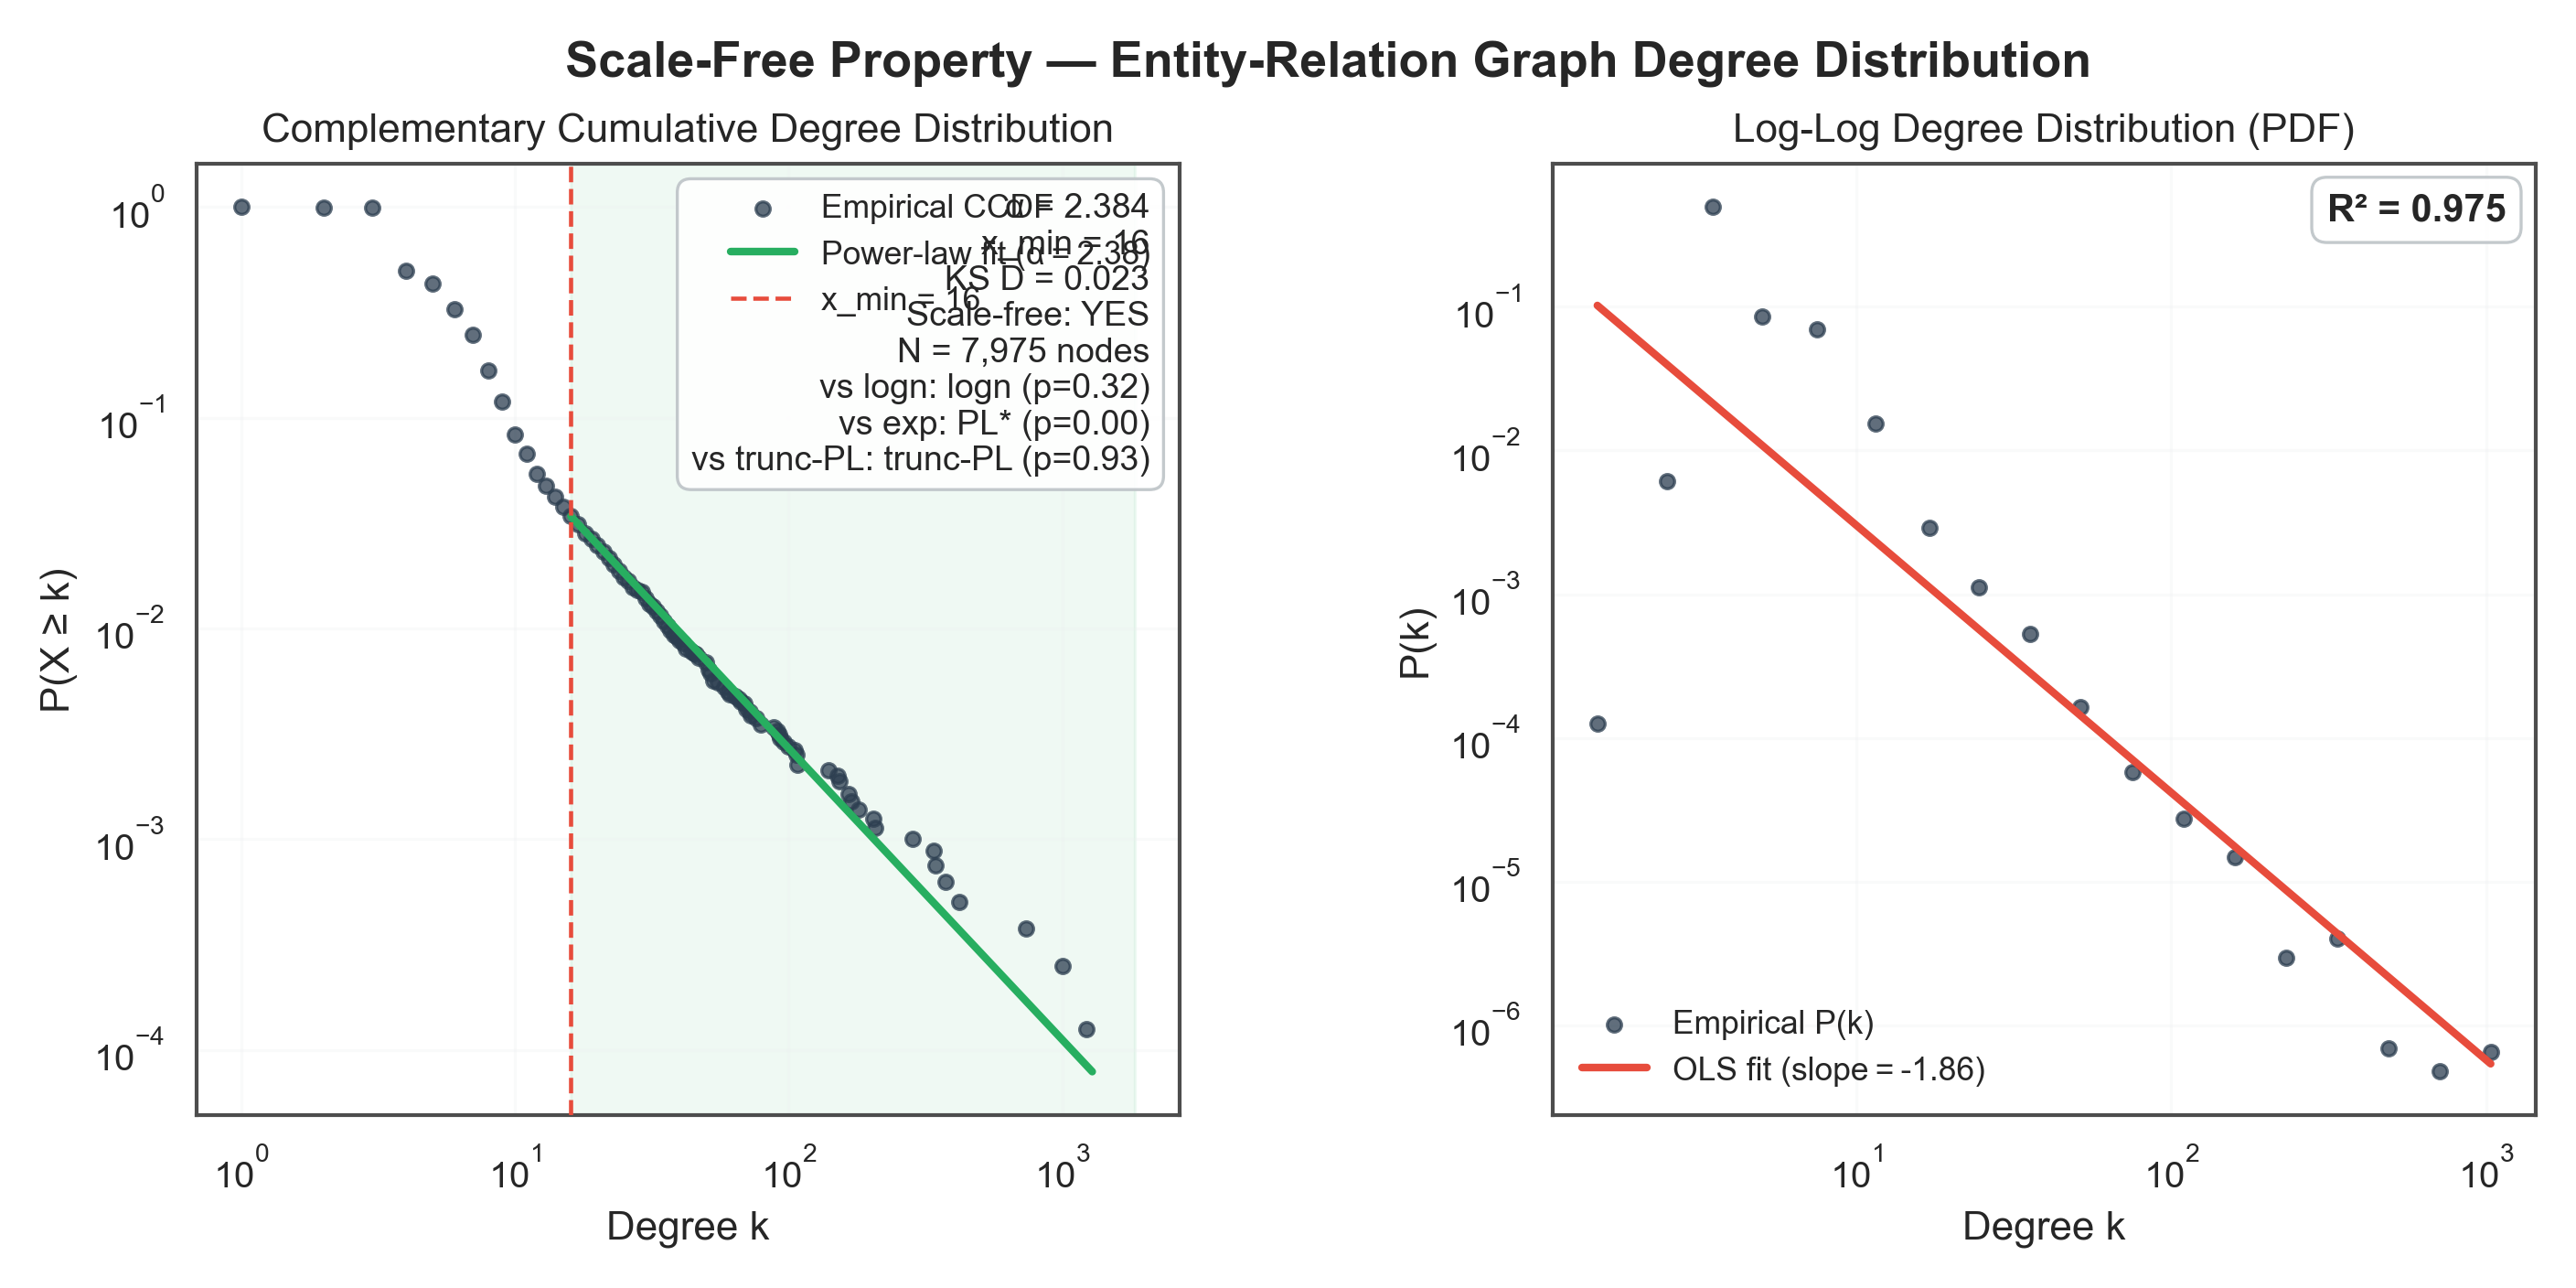
\includegraphics[width=0.80\textwidth]{figs/scale_free_degree_distribution.png}
\caption{Degree distribution of the full-corpus knowledge graph on log--log axes, with the Clauset maximum-likelihood power-law fit ($\alpha=2.38$, $k_{\min}=16$, KS $=0.023$).}
\end{figure}

\hrule

\section{Chapter 3: From Graph to Topics: Community Detection and Summarisation}

\subsection{3.1 Community Detection with the Leiden Algorithm}

With a validated knowledge graph in hand, the task of identifying topics becomes a problem of \emph{community detection}: partitioning the graph into subsets of nodes that are more densely connected internally than they are to the rest of the network. Each resulting community corresponds to a thematically coherent cluster of entities and relationships---the graph-theoretic operationalisation of a topic.

This approach follows the logic of the GraphRAG framework (Edge et al., 2024), which applies community detection to knowledge graphs to generate what the authors call a ``Global Context'': a set of community-level summaries that collectively describe the thematic landscape of an entire corpus. Each community summary is, in effect, a topic. The present work applies the same community-as-topic framework to parliamentary discourse.

The algorithm used is Leiden (Traag, Waltman, \& van Eck, 2019), an iterative method that maximises \emph{modularity}---a quality function measuring the difference between the actual density of edges within detected communities and the density expected under a random null model. A high modularity score indicates that the communities are genuine structural partitions, not statistical accidents. Leiden improves on its predecessor, the Louvain method, by guaranteeing (by construction) that all detected communities are internally well-connected---no disconnected fragments masquerading as a single topic. This is not a cosmetic distinction: Traag et al.\ (2019) show that Louvain can return arbitrarily badly connected communities, with up to 25\% of communities badly connected and up to 16\% actually disconnected when the algorithm is iterated, while Leiden also uncovers higher-modularity partitions and runs faster on hard instances. For a topic model this matters directly---a disconnected ``community'' would correspond to a topic whose constituent entities are not actually related, exactly the artefact the method must avoid.

The Leiden algorithm is configured with a resolution parameter of 0.5, which controls the granularity of the partition (lower values produce fewer, larger communities). The algorithm runs for 2 iterations with a minimum community size of 3 nodes and a fixed random seed of 42 for reproducibility.

\subsubsection{3.1.1 Improving the Partition with node2vec Edge Reweighting}

Applied to an unweighted graph, the Leiden algorithm treats every edge as equally informative about community membership. But in a discourse graph, not all connections carry the same signal. An edge between ``Ukraine'' and ``Russian Aggression''---two entities deeply embedded in the same tightly-knit cluster---is a stronger indicator of community membership than an edge between the hub node ``European Union'' and some peripheral entity it connects to incidentally.

To address this, the pipeline uses node2vec (Grover \& Leskovec, 2016) to learn a structural embedding for every node in the graph, and then uses those embeddings to reweight the edges before community detection. The process has three steps.

\textbf{Step 1: Learning structural embeddings.} node2vec performs biased random walks over the graph and trains a skip-gram model on the resulting sequences of node visits, producing a 128-dimensional vector for every node. Each walk is 20 steps long, and 20 walks are generated per node. With the return parameter $p = 1$ and the in-out parameter $q = 1$ (both at their defaults), the walks balance local neighbourhood exploration with broader traversal. Nodes occupying similar structural positions---belonging to the same tightly-knit cluster, sharing the same neighbours---end up with similar vectors.

\textbf{Step 2: Reweighting edges.} For every edge in the graph, the cosine similarity between the node2vec vectors of its two endpoint nodes is computed. This similarity score becomes the edge's weight. Edges connecting structurally similar nodes receive high weights; edges connecting structurally dissimilar nodes---bridges between clusters, or links from a hub to a distant periphery---receive low weights.

\textbf{Step 3: Weighted community detection.} The Leiden algorithm runs on this reweighted graph. The high-weight edges act as strong ``glue'' that keeps cohesive groups together, while the low-weight edges between clusters are easier for the algorithm to cut. The effect is a sharper, more clearly delineated partition.

This procedure has independent support in the network-science literature. Kov\'{a}cs et al.\ (2024) show that embedding a network and reweighting its links by the geometric proximity of their endpoints ``reinforces intra-community links and weakens inter-community links,'' making communities more easily detectable, and that using this as a preprocessing step improves standard community-detection algorithms; node2vec is among the embeddings they evaluate. The design used here is a single-pass instance of that general idea, applied for the first time (to the author's knowledge) to an LLM-extracted discourse graph.

The empirical result is direct and statistically robust. On the full 7{,}975-node knowledge graph, Leiden achieves a baseline modularity of \textbf{0.702} on the unweighted graph; after node2vec edge reweighting the modularity rises to \textbf{0.812}---an absolute gain of $+0.110$, or $+15.7\%$. Two independent tests confirm this is not an artefact.

First, a \emph{permutation test} rules out that any reweighting would raise modularity: the observed reweighted score is compared against a null distribution of 1{,}000 random edge-weight shufflings. The weighted modularity of 0.812 lies far beyond the 99th percentile of the null (0.726), giving $p<0.001$. The improvement is therefore specific to the topological signal node2vec encodes, not a by-product of reweighting per se.

Second, a \emph{seed-stability analysis} rules out a lucky partition. Repeating each condition across 20 random seeds yields two tight, non-overlapping distributions (Table~\ref{tab:seed}): baseline $0.701 \pm 0.002$ versus weighted $0.812 \pm 0.001$, separated with a Mann--Whitney $p = 3.4\times10^{-8}$ and a Cohen's $d$ of $58.9$. The weakest weighted run still exceeds the strongest baseline run; the reweighting gain is roughly fifty times larger than the seed-to-seed noise. Within the tested parameter settings, node2vec reweighting provides a clear, large, and reproducible lift.

\begin{table}[h]
\centering
\small
\caption{Modularity across 20 random seeds per condition. The two distributions do not overlap.}
\label{tab:seed}
\begin{tabular}{lcc}
\toprule
\textbf{Condition} & \textbf{Mean modularity} & \textbf{Std.\ dev.} \\
\midrule
Baseline (unweighted) & 0.7012 & 0.0024 \\
node2vec-weighted     & 0.8117 & 0.0011 \\
\midrule
Mann--Whitney $U$ test & \multicolumn{2}{r}{$p = 3.4\times10^{-8}$} \\
Cohen's $d$            & \multicolumn{2}{r}{$58.9$} \\
\bottomrule
\end{tabular}
\end{table}

\begin{figure}[h]
\centering
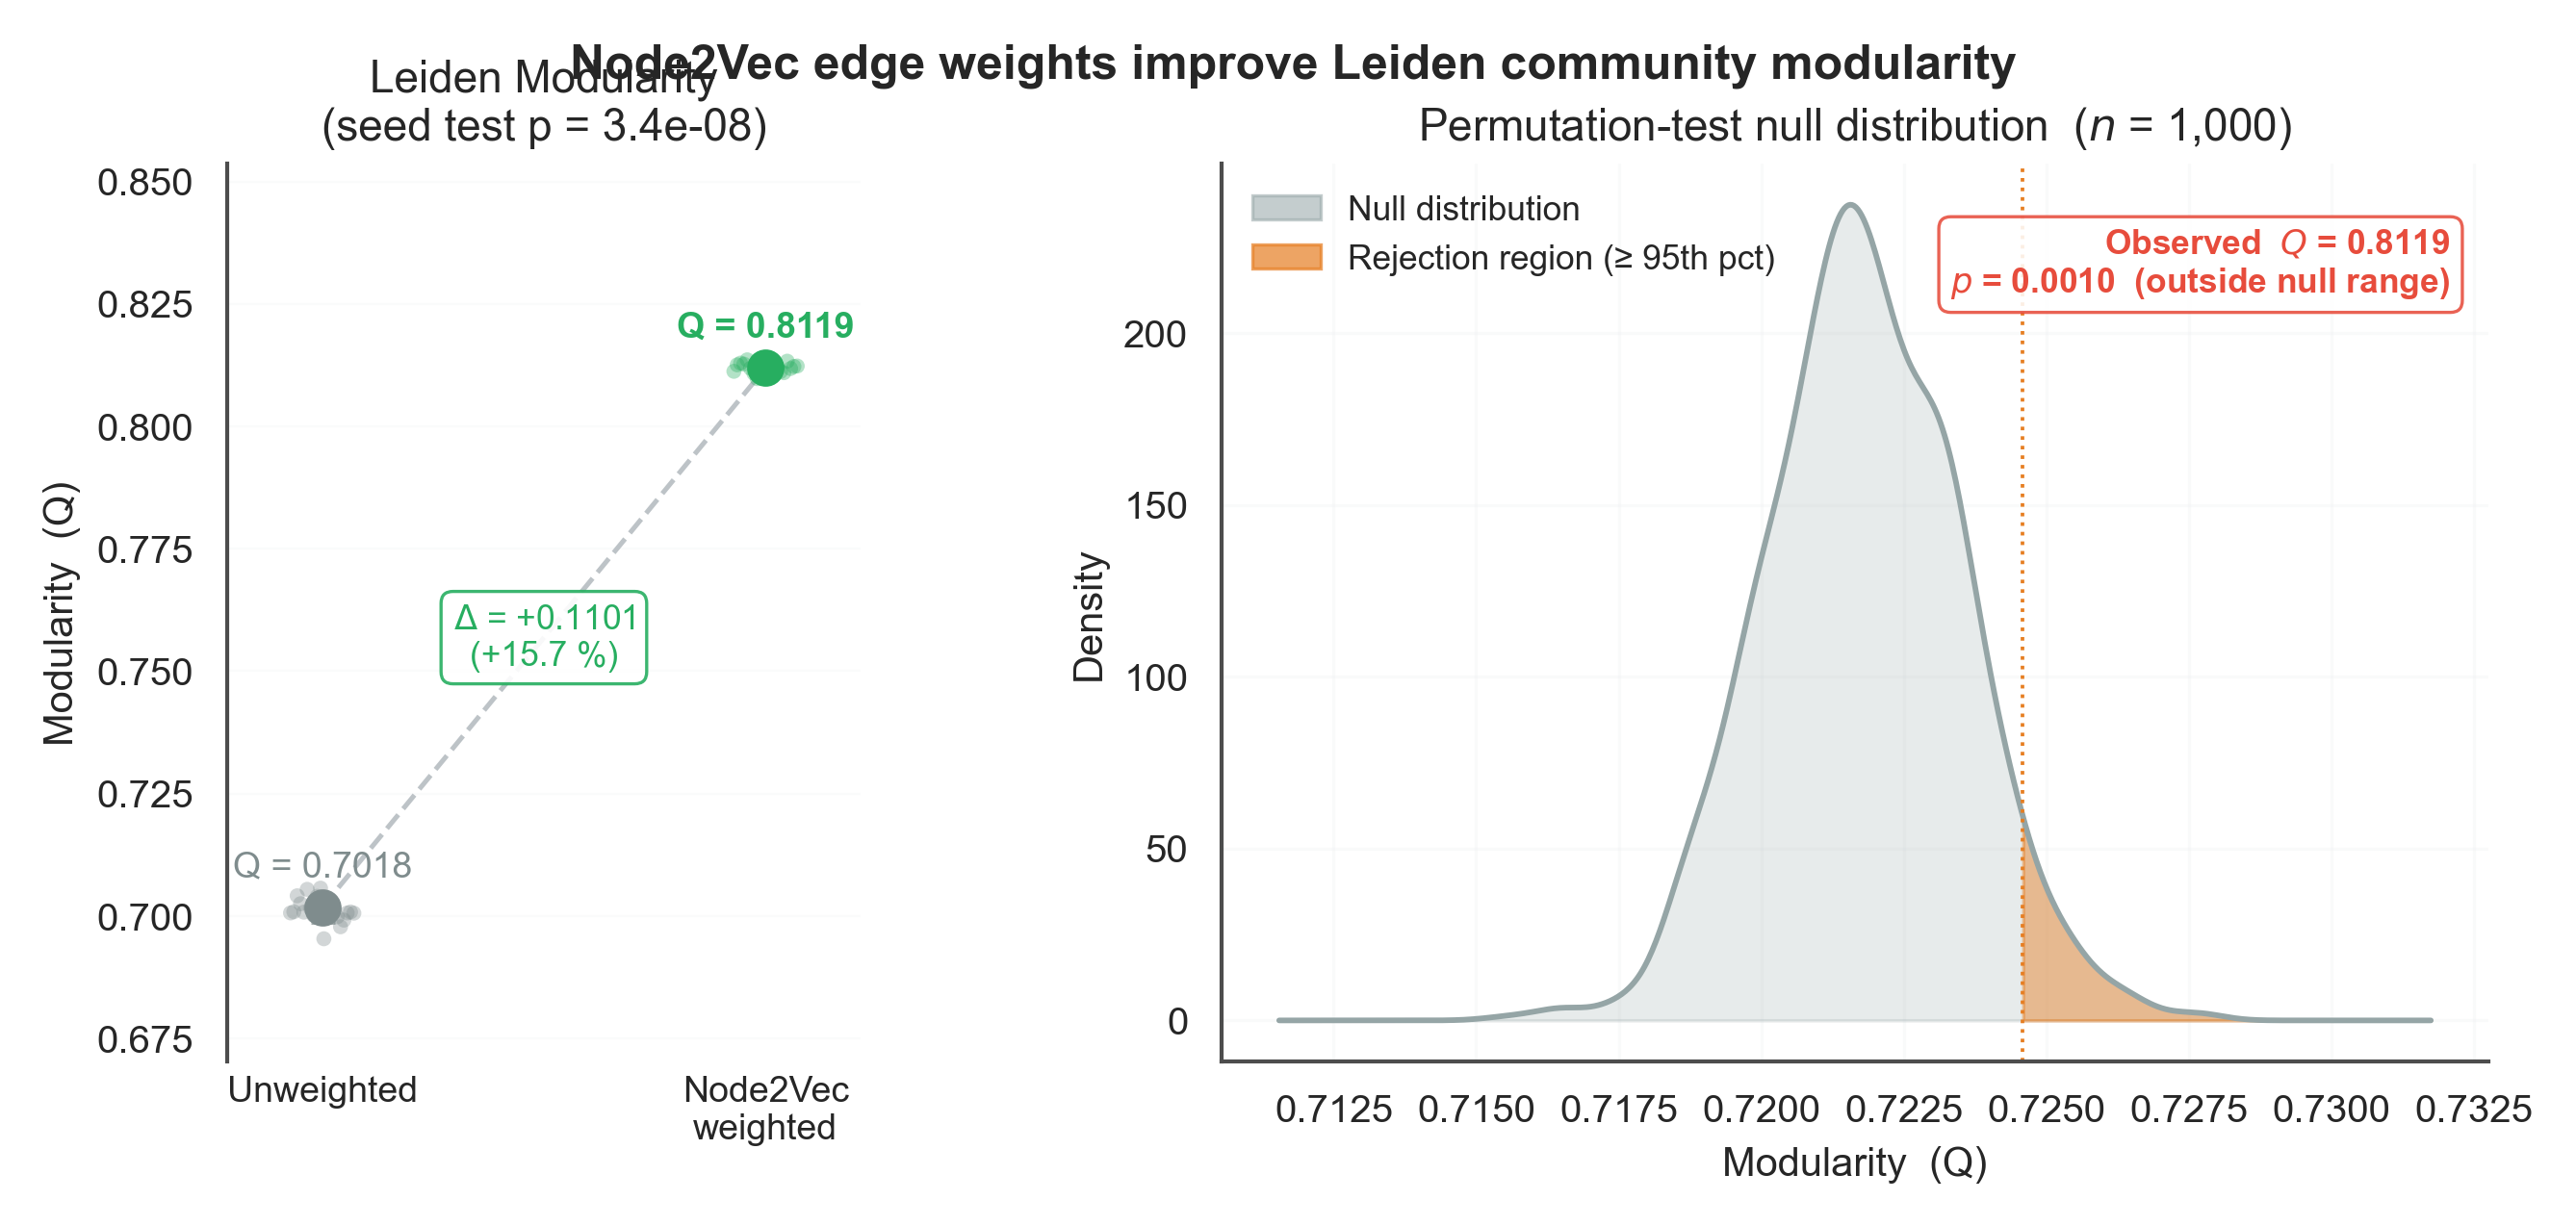
\includegraphics[width=0.80\textwidth]{figs/node2vec_modularity_uplift.png}
\caption{Baseline vs.\ node2vec-weighted modularity across 20 seeds per condition, shown against the permutation null distribution. The two conditions are fully separated.}
\end{figure}

\subsection{3.2 Hierarchical Abstraction}

The Leiden algorithm can be applied recursively. After an initial partition is found, each community can be treated as a new subgraph and partitioned again to reveal finer-grained sub-communities. This produces a nested, multi-resolution view of the thematic landscape: broad themes at the top level (e.g., ``EU's Main Challenges'') decompose into more specific sub-themes (``Energy Crisis,'' ``Inflation,'' ``Disinformation'') at the lower level, mirroring the natural hierarchical organisation of discourse. The reported run yields 99 top-level topics and 683 lower-level subtopics.

\subsection{3.3 Generating Topic Summaries}

The output of community detection is a set of subgraphs---clusters of entities and relationships. While this structure is analytically powerful, it is not immediately interpretable to a reader. The final stage of the pipeline translates each community into a natural language summary using a large language model (Llama-3.3-70B-Instruct via OpenRouter, at temperature 0.0 for deterministic output).

The summarisation follows a strict bottom-up order. Leaf-level communities (subtopics) are summarised first. Their summaries then feed into the summarisation of parent-level communities (topics), ensuring that higher-level summaries are genuine abstractions of their components rather than independent re-descriptions.

For each community, the LLM receives a structured context containing four layers of information:

\begin{enumerate}
  \item \textbf{Community structure}: an enumeration of the community's entities, sorted by degree, accompanied by their ontological types.
  \item \textbf{Relationship network}: the internal edges of the community, formatted as \emph{source--relation--target} triplets.
  \item \textbf{Sub-community summaries}: for parent-level topics, the previously generated summaries of child communities.
  \item \textbf{Textual evidence}: a curated selection of text chunks from the original corpus where the community's entities co-occur.
\end{enumerate}

The LLM is instructed to produce a structured report containing a concise title (3--10 words), an executive summary (3--5 sentences), and detailed findings, each grounded in specific entities, relationships, or textual evidence. This format ensures that every claim in a topic summary is traceable back to the graph structure and the source text.

\hrule

\section{Chapter 4: What the Pipeline Found}

\subsection{4.1 The Discovered Topics}

The pipeline produced 99 communities in total, ranging from a single dominant cluster of 716 entities down to many small, specialised communities of 3 entities each (the median community size is 3). These communities can be grouped into three natural tiers based on their size and thematic scope.

\paragraph{The Core European Discourse.}
The largest communities capture the dominant, cross-cutting themes of the debates:

\begin{itemize}
  \item \textbf{TOPIC\_0}: ``European Union Community Dynamics'' (716 entities). This is the mega-community that absorbs the central discourse: the war in Ukraine, the energy crisis, economic instability, and the EU's commitment to democracy, peace, and security. Its sheer size---more than seven times larger than any other community---reflects the degree to which these topics are interwoven in the speeches.
  \item \textbf{TOPIC\_1}: ``European Union's Response to Global Challenges'' (91 entities). Economic challenges, geopolitical tensions, and social inequalities; the drive toward a Security and Defence Union and reduced fossil-fuel imports.
  \item \textbf{TOPIC\_4}: ``European Integration and Geopolitical Challenges'' (86 entities). Parliamentary debate over the future of the Union, its values, and its stance on geopolitical questions.
  \item \textbf{TOPIC\_2}: ``European Unity and Resilience'' (81 entities). The invasion of Ukraine, economic crises, and the case for strategic autonomy.
  \item \textbf{TOPIC\_3}: ``European Unity Against Russian Aggression'' (79 entities). Solidarity with Ukraine, support for its EU membership, and the war's knock-on effects on global food security.
\end{itemize}

\paragraph{Policy-Specific and National Communities.}
At the middle tier, smaller communities isolate particular policy domains and national perspectives:

\begin{itemize}
  \item \textbf{TOPIC\_11}: ``Greece and the European Union'' (55 entities). Greek economic reform, migration, and the country's relationship with EU institutions.
  \item \textbf{TOPIC\_17}: ``European Integration and Energy Transition'' (55 entities). Energy security threaded through the integration agenda.
  \item \textbf{TOPIC\_16}: ``European Union's Pursuit of Peace and Human Rights'' (48 entities). Values, rights, and the EU's external posture.
  \item \textbf{TOPIC\_23}: ``Luxembourg's Role in European Integration'' (36 entities). A distinctly national angle on the integration project.
  \item \textbf{TOPIC\_21}: ``European Community Dynamics and Strategic Autonomy'' (41 entities). Defence capability and the tension between national independence and collective action.
\end{itemize}

\paragraph{Niche National Debates.}
At the periphery, the smallest communities capture highly specific national issues:

\begin{itemize}
  \item \textbf{TOPIC\_29}: ``Croatian Border Control and European Integration'' (6 entities).
  \item \textbf{TOPIC\_34}: ``Erosion of Democratic Norms in Slovenia'' (5 entities). Attacks on democratic institutions and the `Orbanisation' of Slovenian politics.
  \item \textbf{TOPIC\_41}: ``Finnish Constitution's European Influence'' (4 entities). The influence of Finnish constitutional history on European constitutional law.
  \item \textbf{TOPIC\_51}: ``Protocol Solutions for Northern Ireland'' (3 entities).
  \item \textbf{TOPIC\_59}: ``Criminal Gang Culture in Sweden'' (3 entities).
  \item \textbf{TOPIC\_85}: ``Missing Cypriots: Unresolved Disappearances'' (3 entities).
  \item \textbf{TOPIC\_89}: ``Wagner PMC's Influence in African Regimes'' (3 entities).
  \item \textbf{TOPIC\_90}: ``Bulgargaz and Bota\c{s} Gas Deal'' (3 entities). A specific Bulgaria--Turkey energy agreement.
  \item \textbf{TOPIC\_52}: ``Jean Monnet's Vision for Europe'' (3 entities). A historical-rhetorical aside made by an individual speaker.
\end{itemize}

This three-tier structure---a dense core of interconnected European themes, a middle ring of policy- and country-specific clusters, and a periphery of niche national debates---emerges entirely from the graph topology. It was not prescribed by the ontology or the extraction prompts. The full community-size distribution is shown in Figure~\ref{fig:sizedist}.

\begin{figure}[h]
\centering
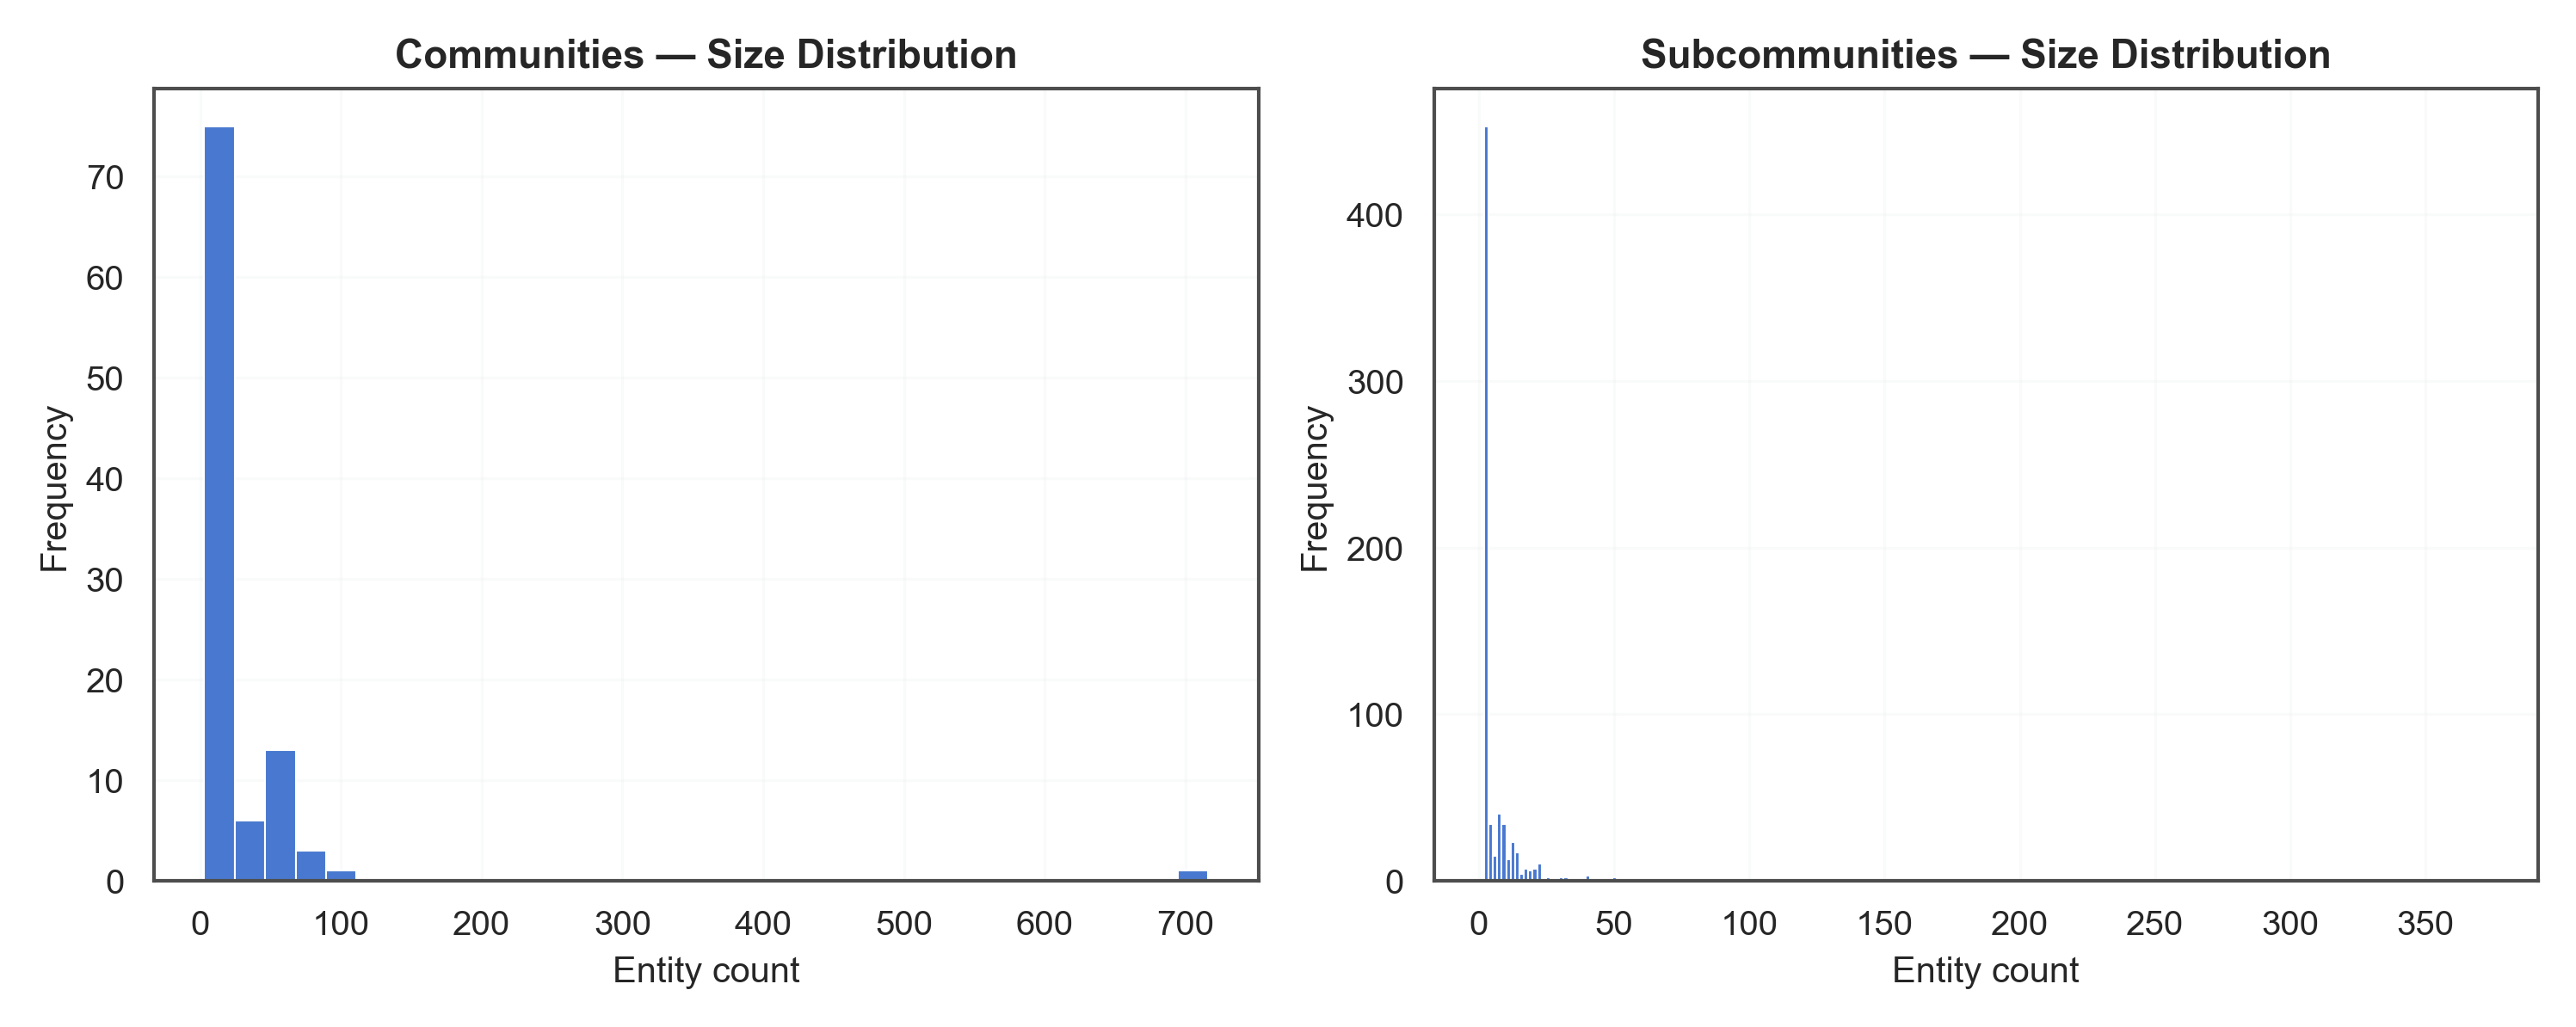
\includegraphics[width=0.74\textwidth]{figs/community_size_distribution.png}
\caption{Community-size distribution of the 99 discovered topics: one dominant 716-entity core, a handful of mid-sized communities, and a long tail of small, specific communities (median size 3).}
\label{fig:sizedist}
\end{figure}

\subsection{4.2 Who Are the Hubs? Centrality in the Knowledge Graph}

The centrality analysis reveals which entities occupy the most structurally important positions in the graph. Table~\ref{tab:centrality} reports the top entities across the standard centrality measures (normalised scores; a dash indicates the entity did not rank in the top reporting threshold for that particular measure).

\begin{table}[h]
\centering
\small
\caption{Top entities by centrality measures (normalised scores), from the canonical full-corpus graph.}
\label{tab:centrality}
\begin{tabular}{lccccc}
\toprule
\textbf{Entity} & \textbf{Degree} & \textbf{Betweenness} & \textbf{Closeness} & \textbf{Eigenvector} & \textbf{PageRank} \\
\midrule
European Union       & 0.147 & 0.032 & 0.050 & 0.143 & 0.0042 \\
European Commission  & 0.091 & 0.021 & 0.043 & 0.068 & 0.0022 \\
Europe               & 0.086 & 0.026 & 0.054 & 0.137 & 0.0071 \\
European Parliament  & 0.038 & 0.009 & ---   & ---   & 0.0015 \\
Ukraine              & 0.023 & 0.009 & 0.050 & 0.120 & 0.0021 \\
Bulgaria             & 0.021 & 0.008 & 0.044 & 0.062 & 0.0011 \\
Greece               & 0.019 & 0.004 & 0.043 & ---   & 0.0013 \\
Cyprus               & 0.016 & 0.002 & 0.043 & 0.063 & ---    \\
Russia               & 0.015 & 0.002 & 0.044 & 0.063 & ---    \\
NATO                 & ---   & ---   & ---   & 0.072 & ---    \\
Democracy            & ---   & ---   & ---   & 0.063 & ---    \\
\bottomrule
\end{tabular}
\end{table}

``European Union'' dominates all measures, which is expected given that the entire corpus is about EU affairs, followed by ``European Commission'' and ``Europe.'' More interesting are the secondary hubs. ``Ukraine'' has a high eigenvector centrality (0.120)---meaning it is connected to other highly connected nodes---despite a much lower raw degree than its eigenvector rank would suggest. This reflects a structural asymmetry: national actors such as Greece and Bulgaria appear frequently because their leaders gave particularly detailed speeches, while Ukraine is structurally central because it connects to the dominant crisis themes that run through \emph{every} speech.

Most tellingly, ``NATO'' (eigenvector 0.072) and ``Democracy'' (0.063) rank among the top entities by eigenvector centrality despite not registering in the top ranks by raw degree at all. These entities matter not because of their own direct connections but because they sit at the intersection of other highly connected themes---NATO links defence, enlargement, and collective security; democracy links values, rule of law, and the critique of authoritarian drift. This is precisely the kind of structural insight that a graph-based approach can surface but a word-frequency analysis would miss.

\subsection{4.3 Validation Against the EPRS Ground Truth}

The central question is whether the pipeline's topics correspond to those identified by human experts. This can be stated both quantitatively and qualitatively.

\paragraph{Quantitative coverage.}
Embedding each of the six recurring EPRS themes and matching it against all 99 community summaries by cosine similarity, \emph{every} EPRS theme finds a corresponding community: coverage is $100\%$ (6/6), with a mean best-match similarity of $0.444$ (median $0.444$, minimum $0.095$). Table~\ref{tab:eprs} reports, for each theme, its single strongest community match and the number of communities for which it is the nearest theme. The distribution of matches is itself informative: five of the six themes are the nearest theme for 18--21 communities apiece, confirming that these are the cross-cutting spine of the corpus, whereas ``the value of EU membership''---an abstract framing rather than a concrete subject---is the nearest theme for only two communities. A mean similarity of 0.44 signals a thematic rather than a verbatim correspondence, which is appropriate: the pipeline recovers the EPRS's themes as \emph{regions} of its topic landscape, not as identical labels. The full theme-by-community similarity structure is visualised in Figure~\ref{fig:gtheat}.

\begin{table}[h]
\centering
\small
\caption{Best-matching pipeline community for each of the six recurring EPRS themes (canonical run). ``Mapped'' counts how many of the 99 communities take this theme as their nearest.}
\label{tab:eprs}
\begin{tabular}{p{4.3cm}p{5.0cm}cc}
\toprule
\textbf{EPRS theme} & \textbf{Best-matching community} & \textbf{Sim.} & \textbf{Mapped} \\
\midrule
Next steps in EU integration     & TOPIC\_8 EU's Future and Challenges         & 0.74 & 20 \\
The importance of EU unity        & TOPIC\_12 European Unity and Cooperation    & 0.73 & 21 \\
The main challenges facing the EU & TOPIC\_1 EU's Response to Global Challenges  & 0.69 & 19 \\
Defending EU values               & TOPIC\_71 Defenders of Liberal Democracy    & 0.66 & 18 \\
Delivering for EU citizens        & TOPIC\_9 European Community Dynamics         & 0.64 & 19 \\
The value of EU membership        & TOPIC\_30 Integration and Market Balance    & 0.51 & 2  \\
\bottomrule
\end{tabular}
\end{table}

\begin{figure}[h]
\centering
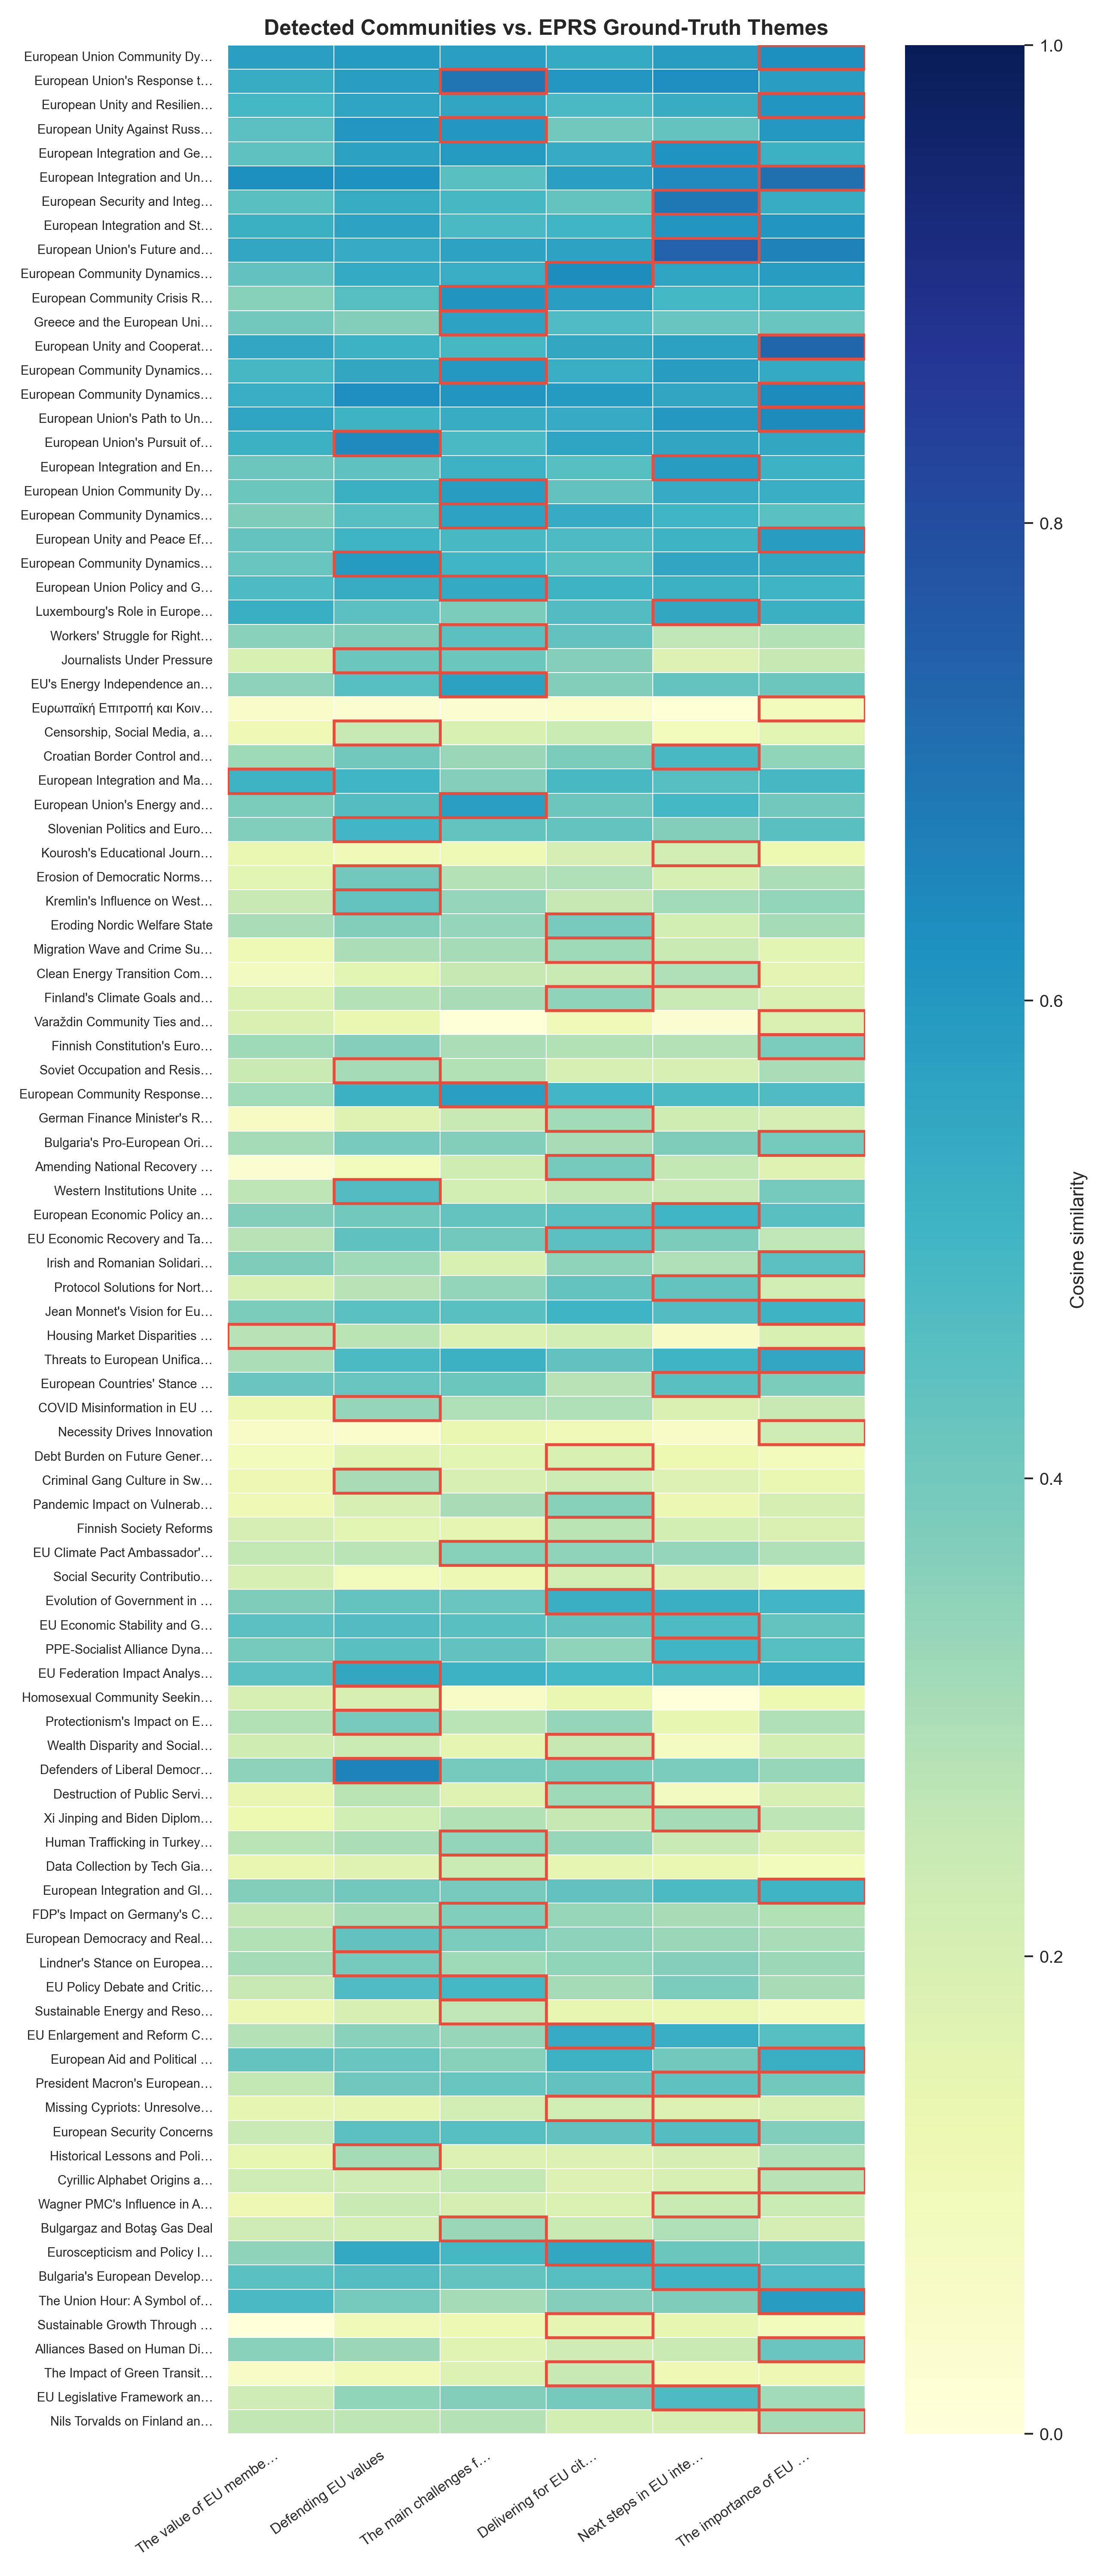
\includegraphics[width=0.92\textwidth]{figs/ground_truth_alignment_heatmap.png}
\caption{Cosine-similarity heatmap of community summaries against the six EPRS themes. Every theme finds at least one strong community match, giving 100\% coverage.}
\label{fig:gtheat}
\end{figure}

\paragraph{Qualitative mapping.}
The pipeline does not produce a clean one-to-one correspondence with the EPRS categories---nor should it, since the EPRS categories are analyst-defined macro-themes while the pipeline communities are algorithmically derived from graph topology. Instead, the alignment is many-to-one: each EPRS category maps to multiple communities at different levels of granularity, consistent with the hierarchical structure of the graph partition.

\emph{Ukraine and the dominant discourse.} The EPRS reports that Ukraine was the single most prominent topic, discussed by all 13 speakers and receiving 14\% of total attention. In the pipeline's output, TOPIC\_0 (716 entities) is overwhelmingly dominated by Ukraine, Russia, sanctions, energy dependency, and EU unity, and TOPIC\_3 (``European Unity Against Russian Aggression,'' 79 entities) isolates the war response specifically. The mega-community's size---more than seven times any other---reflects the degree to which the Ukraine crisis pervades the entire corpus, matching the EPRS finding that Ukraine was the defining context of all the debates.

\emph{Energy as a cross-cutting theme.} The EPRS identifies energy as the second-most discussed policy area. In the knowledge graph, energy does not form a single community but appears across many: TOPIC\_17 (energy transition and integration), TOPIC\_26 (``EU's Energy Independence and Resilience''), TOPIC\_31 (``European Union's Energy and Climate Strategy''), TOPIC\_90 (a specific Bulgaria--Turkey gas deal), and woven through the core communities. This fragmentation reflects a genuine property of the discourse: energy is discussed not as a standalone topic but as a dimension of nearly every other debate---security, climate, economic stability, national policy.

\emph{National policies.} The EPRS notes that national policies were driven primarily by the speeches of Mitsotakis and Christodoulides. The pipeline isolates these national concerns with fine granularity: TOPIC\_11 (``Greece and the European Union,'' 55 entities) captures the Greek agenda; TOPIC\_34 captures Slovenian democratic erosion; TOPIC\_29 the Croatian border question; TOPIC\_85 the unresolved case of missing Cypriots; and TOPIC\_51 the Northern Ireland protocol. The pipeline does not merely identify ``national policies'' as a category---it separates them into distinct, country-specific communities, a level of granularity the EPRS report does not attempt.

\emph{What the pipeline surfaced that the EPRS did not emphasise.} Several communities correspond to arguments the EPRS records only in passing or not at all: TOPIC\_52 (Jean Monnet's founding vision), TOPIC\_88 (the origins of the Cyrillic alphabet, raised by a Bulgarian speaker), and TOPIC\_89 (the Wagner group's influence in Africa). These are niche arguments by individual speakers, too small to register as ``topics'' in a macro analysis but structurally distinct enough for Leiden to separate. Whether they qualify as genuine ``topics'' or merely as isolated anecdotes is a matter of interpretation---but the pipeline's ability to surface them is itself informative.

\subsection{4.4 Similarity Analysis: The Shape of the Topic Landscape}

The pairwise cosine-similarity distribution of the community summaries provides a bird's-eye view of the topic landscape. It is unimodal and centred just below 0.5: subtopic-level pairs have mean $0.466$ (standard deviation $0.153$, over 232{,}903 pairs), and the coarser topic-level pairs have mean $0.440$ (standard deviation $0.128$, over 2{,}016 pairs). The spread runs from near-orthogonal pairs ($\approx 0.07$) to near-duplicates ($\approx 0.95$).

This shape is what one would expect from a corpus unified by its subject (European politics during a shared set of crises) but internally differentiated by national perspective and policy domain. If the topics were entirely unrelated, the distribution would concentrate near zero; if the model had found no meaningful differentiation, it would compress near 1.0. The observed centre near 0.47 sits between these extremes, reflecting a genuine balance of shared context and sub-thematic variation. A formal Shapiro--Wilk test rejects strict normality (subtopics $p \approx 10^{-21}$), but this is expected---at hundreds of thousands of pairs the test rejects almost any empirical distribution; the defensible and sufficient claim is that the distribution is symmetric and single-peaked.

\begin{figure}[h]
\centering
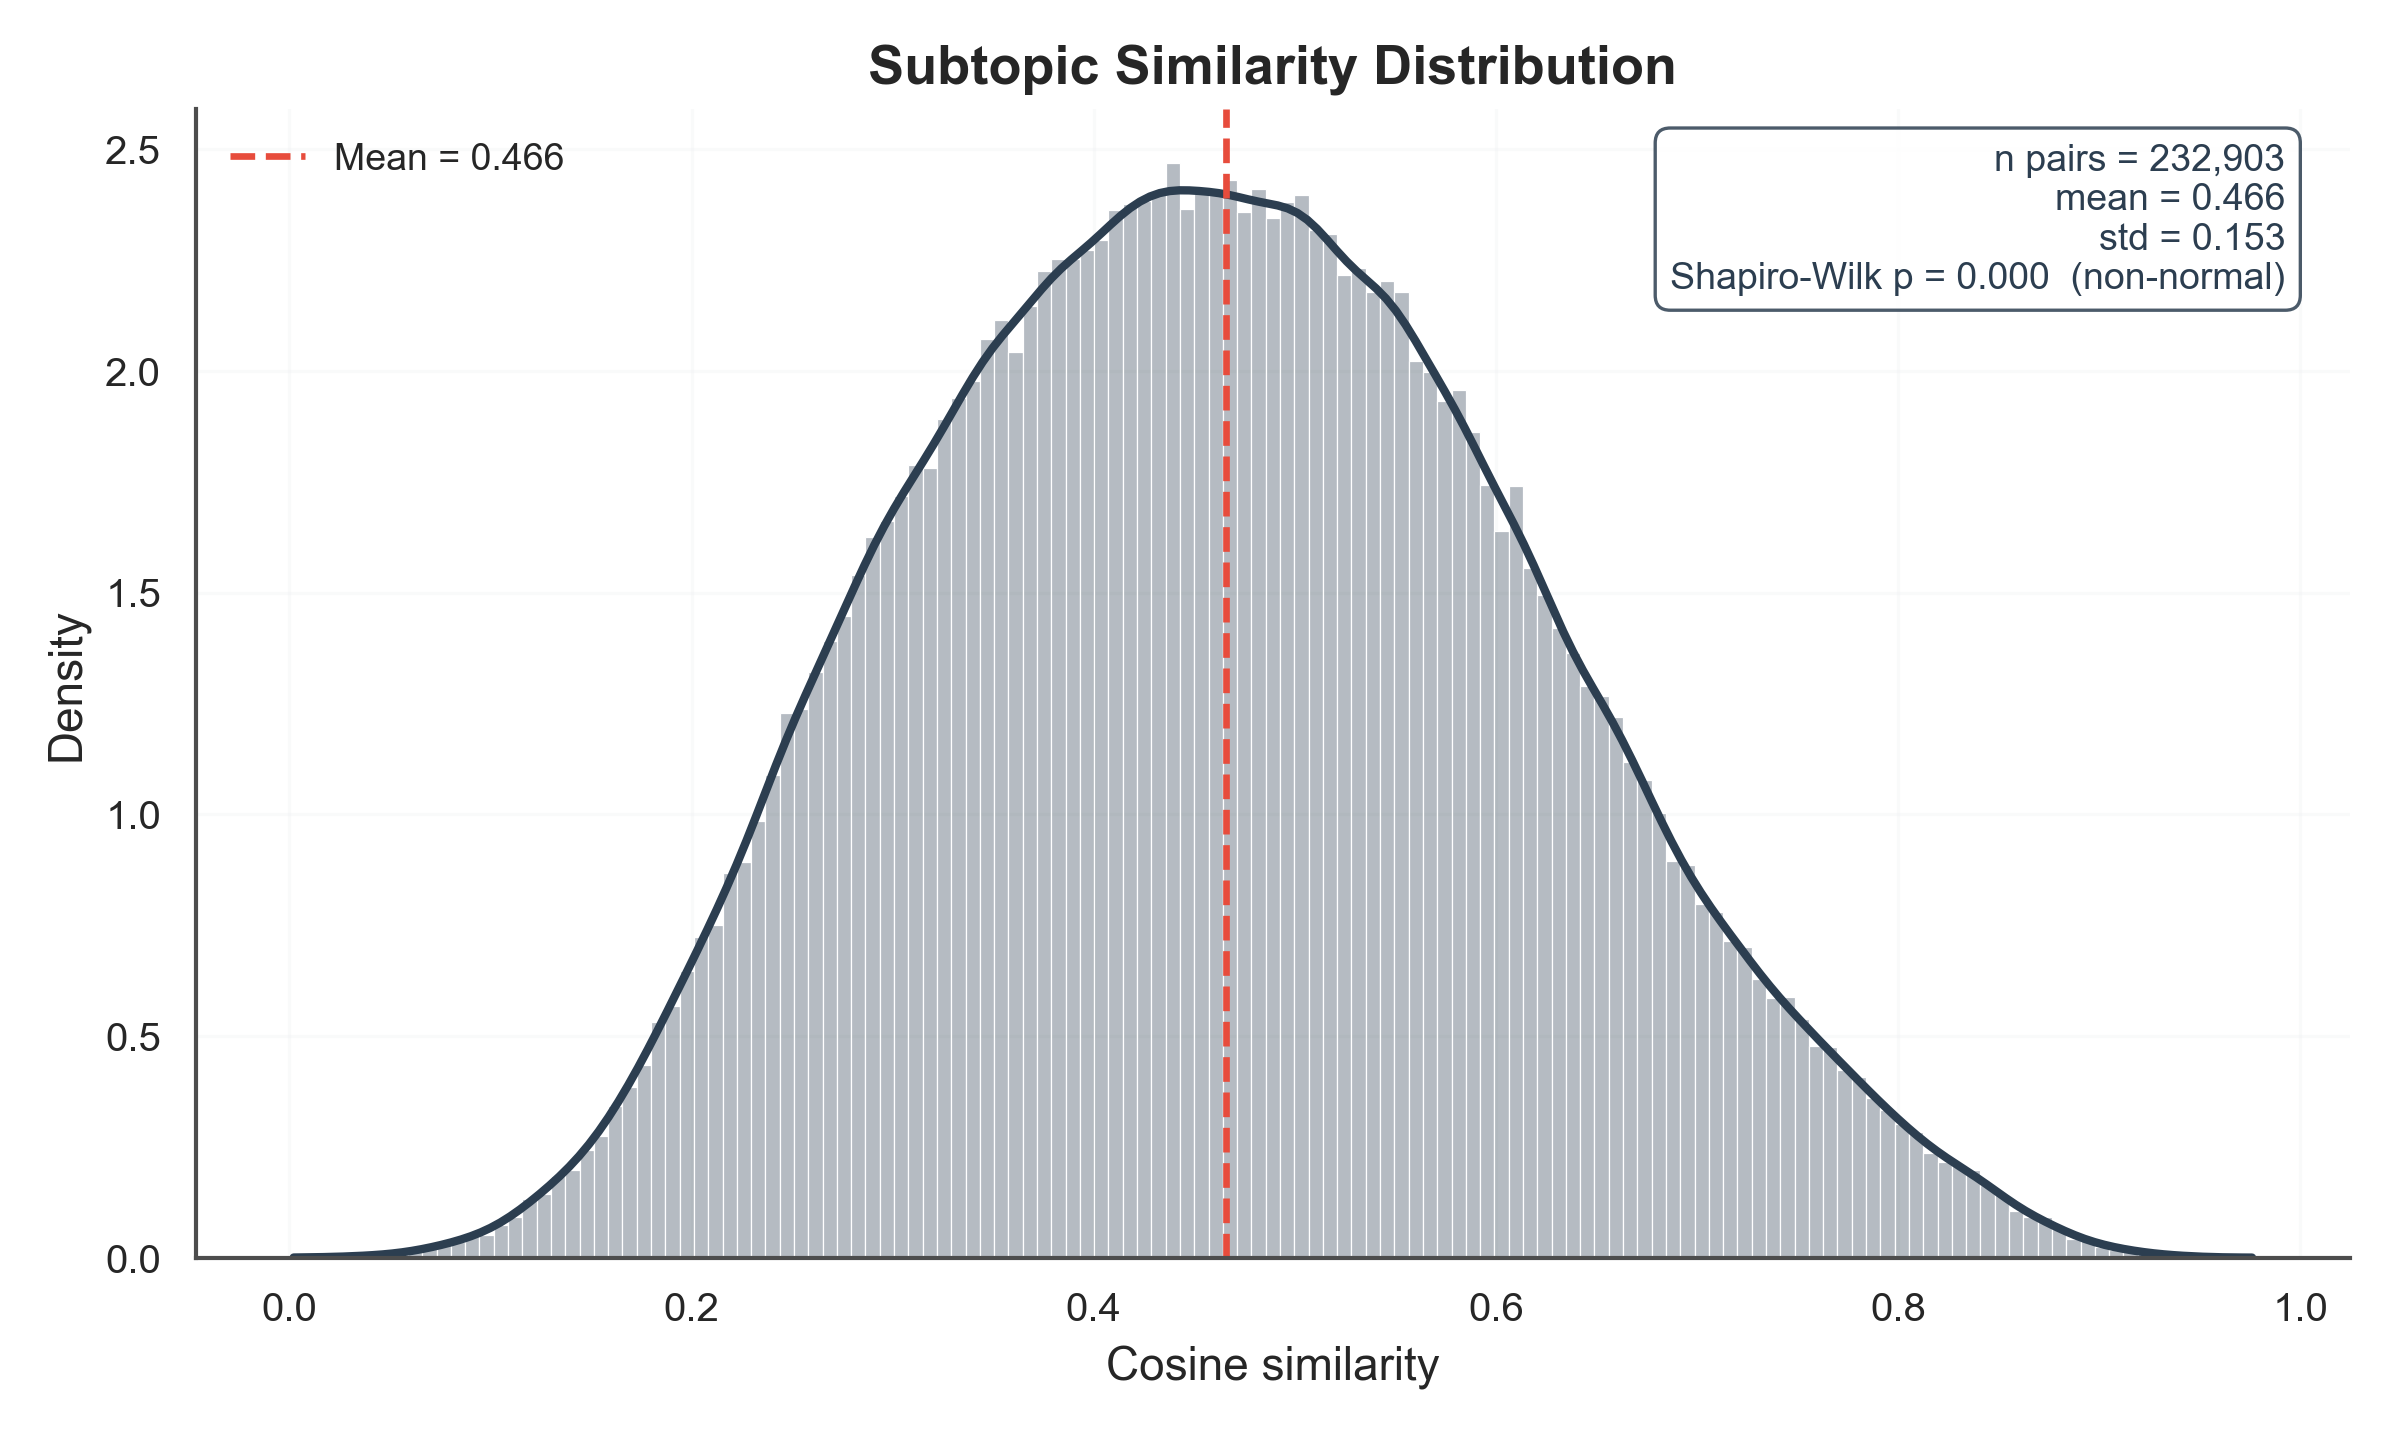
\includegraphics[width=0.74\textwidth]{figs/subtopic_similarity_distribution.png}
\caption{Pairwise cosine-similarity distribution of the 683 subtopic summaries (232{,}903 pairs, $\mu = 0.466$): unimodal and centred just below 0.5.}
\end{figure}

The tails map onto the three-tier structure. The right tail (similarity $\gtrsim 0.6$) corresponds to the core European topics---the Ukraine/energy/security/unity cluster---which share vocabulary, argumentative structure, and entities across communities. The left tail (similarity $\lesssim 0.25$) corresponds to the niche national debates: the Bulgarian gas deal, the Cypriot disappearances, the Northern Ireland protocol. These pairs are semantically distant from the core discourse, confirming that Leiden has successfully separated them.

\subsection{4.5 Honest Limitations: Structural Coherence vs.\ Semantic Overlap}

An important caveat must be stated directly. While Leiden achieves high modularity (0.812), meaning the communities are \emph{structurally} well-defined, their \emph{semantic} distinctiveness is limited. Computing silhouette scores over the entities' semantic embeddings, labelled by community, gives persistently negative values: $-0.264$ at the community level (99 clusters) and $-0.383$ at the subcommunity level (683 clusters), with a global mean intra-community cosine similarity of just $0.235$. A negative silhouette means entities are, on average, closer in embedding space to entities in \emph{other} communities than to those in their own.

This is not a failure of the model; it is a direct and honest measurement. Leiden partitions on \emph{graph topology}---patterns of entity co-occurrence and relation---not on embedding proximity. The negative silhouette therefore confirms that the topological community structure is \emph{not} reducible to semantic distance in embedding space, which is precisely the rationale for taking a graph-based rather than an embedding-clustering approach. When 13 EU leaders discuss the same crises using overlapping vocabularies, their arguments naturally project into overlapping regions of semantic space; the graph nonetheless recovers distinct structural communities by attending to \emph{how} entities are connected rather than \emph{what words} describe them. A model that reported clean, well-separated semantic clusters from this corpus would be more misleading than one that honestly reflects the overlap. (Measuring silhouette instead over the node2vec structural embeddings would quantify topological compactness directly and is the metric more naturally paired with the modularity result of \S3.1.1.)

\subsection{4.6 Baseline Comparison: Classical LDA on the Same Corpus}

The claim that a structural approach helps only carries weight against a probabilistic baseline on identical data. To provide one, Latent Dirichlet Allocation (Blei, Ng \& Jordan, 2003) was trained on exactly the same input: the corpus was segmented with the same character-based splitter the graph pipeline uses (512 characters, 64 overlap), yielding 2{,}083 documents, and standard preprocessing (stop-word and procedural-term removal, extreme-frequency filtering) produced a 2{,}403-word vocabulary. LDA models were fitted with Gensim across a range of topic counts, $k \in \{6, 10, 20, 50, 99\}$, and each model was evaluated on two axes: intrinsic $C_v$ topic coherence---the standard automatic coherence measure of R\"{o}der, Both \& Hinneburg (2015)---and, crucially, the \emph{identical} EPRS ground-truth alignment metric applied to the graph communities in \S4.3, with each LDA topic represented by its 15 highest-probability words. Because the alignment procedure is the same (embed the topic representation, match to the six EPRS theme descriptions by cosine similarity), the two methods can be compared head to head.

\begin{table}[h]
\centering
\small
\caption{LDA baseline across topic counts $k$, evaluated on the same corpus and the same EPRS alignment metric as the graph pipeline. The final row is the graph-based result from \S4.3.}
\label{tab:lda}
\begin{tabular}{lcccc}
\toprule
\textbf{Model} & \textbf{$C_v$ coherence} & \textbf{EPRS coverage} & \textbf{Themes matched} & \textbf{Mean best-match sim.} \\
\midrule
LDA, $k=6$   & 0.353 & 50\%  & 3/6 & 0.355 \\
LDA, $k=10$  & 0.326 & 67\%  & 4/6 & 0.392 \\
LDA, $k=20$  & 0.340 & 67\%  & 4/6 & 0.390 \\
LDA, $k=50$  & 0.329 & 100\% & 6/6 & 0.369 \\
LDA, $k=99$  & 0.340 & 83\%  & 5/6 & 0.351 \\
\midrule
\textbf{Graph pipeline (99 topics)} & --- & \textbf{100\%} & \textbf{6/6} & \textbf{0.444} \\
\bottomrule
\end{tabular}
\end{table}

Three findings emerge (Table~\ref{tab:lda}, Figure~\ref{fig:lda}). First, \textbf{at matched granularity the graph pipeline dominates}. With 99 topics apiece, LDA recovers only five of the six EPRS themes (83\% coverage) at a mean best-match similarity of 0.351, whereas the graph pipeline recovers all six (100\%) at 0.444. The graph approach is simultaneously more complete and more cleanly aligned.

Second, \textbf{LDA reaches full coverage only at a carefully chosen $k$, and never matches the alignment quality}. Coverage is non-monotonic in $k$---it climbs to 6/6 at $k=50$ but falls back to 5/6 at $k=99$---which is itself a symptom of the instability of probabilistic topic assignment on a corpus with heavily overlapping vocabulary. Even at its best ($k=50$), LDA's mean best-match similarity of 0.369 remains well below the graph's 0.444: its topics land on the EPRS themes less precisely because they are distributions over a shared vocabulary rather than distinct entity-relational structures.

Third, and most tellingly, \textbf{LDA systematically fails on the hardest theme}. ``The value of EU membership''---an abstract framing whose vocabulary (single market, prosperity, solidarity) is diffused across every other theme---is the nearest theme for \emph{zero} LDA topics at $k=99$ and for at most one at any $k$. The graph pipeline, by contrast, isolates two communities for it. Where LDA reaches full coverage (at $k=50$) it does so by scattering topics unevenly---16 onto ``delivering for citizens,'' 14 onto ``challenges,'' but only 1 onto ``value of membership''---rather than by genuinely resolving the diffuse theme. This is precisely the regime, flagged in \S2.1, where bag-of-words methods struggle: when every speaker draws on the same lexicon, word co-occurrence cannot separate themes that the relational structure of the discourse keeps distinct.

This failure mode is well documented. Because LDA infers topics from document-level word co-occurrence, it degrades when that co-occurrence signal is sparse or when the vocabulary is heavily shared across topics---the motivation for co-occurrence-aggregating variants such as the Biterm Topic Model (Yan et al., 2013) and, more broadly, for the family of short-text topic models surveyed by Qiang et al.\ (2022). The relevant property here is not literal document length---parliamentary speeches are long---but the same underlying pathology: after chunking, and given a lexicon in which ``Europe,'' ``crisis,'' ``energy,'' and ``unity'' recur in almost every passage, the per-context co-occurrence statistics LDA relies on are precisely the ones that blur. It should be said plainly that this degradation is not universal: Albalawi et al.\ (2020) found LDA to yield \emph{more} coherent topics than several alternatives on some corpora, so the honest claim is that LDA \emph{tends} to struggle in the high-overlap regime, not that it always does---and the head-to-head result above is offered as evidence for this specific corpus rather than as a general verdict. A final caveat applies to the coherence axis itself: automatic coherence scores such as $C_v$ are known to correlate imperfectly with human judgement (Hoyle et al., 2021), which is exactly why the primary comparison in this thesis rests on alignment to an independent expert ground truth rather than on coherence alone.

\begin{figure}[h]
\centering
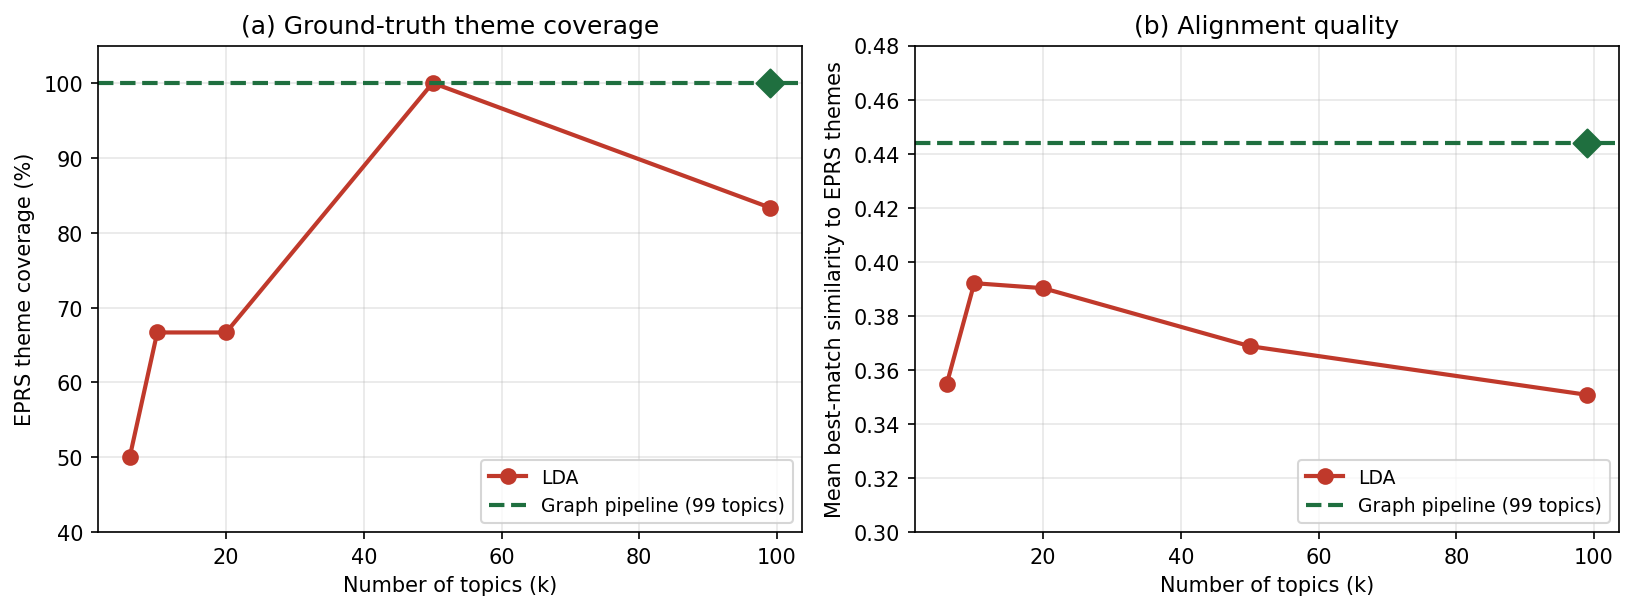
\includegraphics[width=0.95\textwidth]{figs/lda_comparison.png}
\caption{LDA baseline versus the graph pipeline on the same corpus and the same EPRS alignment metric. (a) Theme coverage: LDA reaches full coverage only at $k=50$ and falls back at $k=99$; the graph pipeline covers all six themes. (b) Alignment quality: LDA's mean best-match similarity peaks below the graph pipeline's at every $k$.}
\label{fig:lda}
\end{figure}

Beyond the metrics, the two methods differ in interpretability. An LDA topic is a ranked word list; several of those produced here are difficult to read as coherent themes (for example, one $k=20$ topic reads \emph{prime, minister, government, defense, cooperation, right, realistic, politics, countries, security, \ldots}, and untranslated fragments and procedural terms such as ``blue card'' surface as topic words). A graph community, by contrast, comes with a structured summary, a ranked list of typed entities, and the source chunks in which they co-occur---every claim traceable back to the graph and the text. On this corpus, then, the graph-based approach is not merely competitive with LDA; it is more complete against the expert ground truth, more precisely aligned, more stable across granularities, and more interpretable. This is the central empirical argument of the thesis.

\hrule

\section{Chapter 5: Conclusion}

\subsection{5.1 What This Thesis Found}

This thesis explored whether building a knowledge graph from parliamentary text and detecting communities within it could produce meaningful, interpretable topics. The results suggest that it can, with some important qualifications.

The pipeline transforms unstructured text into a knowledge graph through a sequence of concrete steps: per-chunk ontology matching against the EU's CDM vocabulary family, ontology-guided LLM triplet extraction, multi-stage entity resolution, and graph assembly. The resulting graph (7{,}975 nodes, 4{,}841 resolved entities) exhibits a heavy-tailed, scale-free degree distribution (Clauset exponent $\alpha \approx 2.38$, KS $=0.023$), consistent with organically grown networks and suggesting the extraction preserved genuine discourse structure. node2vec edge reweighting lifts the Leiden algorithm's modularity from 0.702 to 0.812 ($+15.7\%$), a gain confirmed by a permutation test ($p<0.001$) and a 20-seed stability analysis (Cohen's $d = 58.9$). The 99 resulting communities, when summarised by a large language model, recover all six of the EPRS's recurring themes (100\% coverage).

Three observations stand out. First, the pipeline separates the dominant pan-European discourse (Ukraine, energy, unity) from niche national debates (Croatian borders, Slovenian democratic backsliding, the Northern Ireland protocol)---a three-tier structure that matches the EPRS's distinction between cross-cutting themes and speaker-specific concerns. Second, the centrality analysis reveals structural roles that go beyond word frequency: ``NATO'' and ``Democracy'' are structurally central by eigenvector centrality despite modest raw degree, because they connect to other highly connected themes. Third, energy does not form a single topic but is distributed across many communities, faithfully reflecting its cross-cutting nature in the debates. A head-to-head comparison against LDA on the same corpus (\S4.6) makes the case concrete: the structural approach recovers the expert themes more completely, aligns to them more precisely, and does so more stably across granularities than the probabilistic baseline.

\subsection{5.2 What It Contributes}

The primary contribution is methodological: a working pipeline that translates graph topology into auditable, structured topic reports. Unlike probabilistic models that produce opaque word distributions, this approach generates explicit knowledge structures where every claim in a topic summary can be traced to specific entities, relationships, and source text. This transparency is particularly valuable in domains like political science and policy analysis, where interpretability matters.

The contribution sits within a clear lineage but occupies a gap in it. The idea that topics can be recovered as network communities is established for \emph{word} graphs---Gerlach, Peixoto \& Altmann (2018) give it a formal footing by showing LDA to be a special case of a stochastic block model, and Chowdhury et al.\ (2023) demonstrate community detection on word-association graphs competing with probabilistic models. Separately, GraphRAG (Edge et al., 2024) established the machinery of LLM-extracted \emph{entity} graphs with Leiden communities and LLM summaries, but as a retrieval-and-summarisation system evaluated on question answering, not as a topic model measured against expert themes. This thesis joins the two strands: it applies the community-as-topic principle to an LLM-built entity knowledge graph and evaluates it as a topic model, quantitatively, against an independent expert analysis of the same corpus. To the author's knowledge, that specific evaluation---graph-community topics versus LDA, both scored on alignment to the same expert ground truth---has not previously been reported for political discourse.

The node2vec reweighting step is worth highlighting. The idea of using topological embeddings to improve community detection is not new, but the measurable, statistically validated lift it provides on this corpus ($+15.7\%$ modularity, $p<0.001$, $d=58.9$) demonstrates its practical value: it transforms the Leiden partition from adequate to substantially sharper by making the community structure more legible to the algorithm.

The thesis also offers a candid view of the approach's limitations in the context of highly cohesive political discourse. The negative silhouette scores are not a failure of the model---they are an honest measurement of the degree to which European parliamentary debate is semantically interconnected, and a demonstration that the graph captures structure that semantic embeddings alone would miss.

\subsection{5.3 Limitations and Directions for Future Work}

Several limitations should be noted directly. The semantic overlap between topics remains a challenge: while the communities are structurally distinct, their summaries often mention the same entities. Developing post-processing methods to merge structurally separate but semantically identical communities would be a natural next step. Relatedly, the semantic entity-resolution threshold (cosine 0.95) occasionally over-merges distinct concepts; a stricter or type-aware merge rule would sharpen the entity set.

The pipeline was tested on a single, relatively small corpus (13 speeches). It would be interesting to see how the approach scales to larger corpora, to debates in other languages, or to domains outside European politics where the topics may be more sharply differentiated. The LDA comparison of \S4.6 could likewise be broadened---to neural topic models such as BERTopic, or to human-judged coherence---to further characterise where the structural advantage is largest.

The resolution parameter of the Leiden algorithm (set to 0.5 here) strongly influences the number and size of communities. A systematic exploration of resolution values, perhaps using stability analysis across multiple resolutions, could provide a more principled basis for choosing it.

Finally, the current pipeline is static: it produces a single snapshot of the discourse. Extending it to track how topics emerge, merge, and evolve as new speeches are added---a dynamic or temporal analysis---could yield insights into political consensus formation that a static analysis cannot capture.

\hrule

\subsection*{References}

Albalawi, R., Yeap, T. H. \& Benyoucef, M. (2020) `Using topic modeling methods for short-text data: A comparative analysis', Frontiers in Artificial Intelligence, 3, 42.

Barab\'{a}si, A.-L. \& Albert, R. (1999) `Emergence of scaling in random networks', Science, 286(5439), pp. 509--512.

Blei, D. M., Ng, A. Y. \& Jordan, M. I. (2003) `Latent Dirichlet Allocation', Journal of Machine Learning Research, 3, pp. 993--1022.

Broido, A. D. \& Clauset, A. (2019) `Scale-free networks are rare', Nature Communications, 10, 1017.

Chowdhury, M. A. R., Ahmed, M. T., Sadeque, F. \& Yanhaona, M. N. (2023) `Topic modeling using community detection on a word association graph', Proceedings of the 14th International Conference on Recent Advances in Natural Language Processing (RANLP), pp. 900--910.

Clauset, A., Shalizi, C. R. \& Newman, M. E. J. (2009) `Power-law distributions in empirical data', SIAM Review, 51(4), pp. 661--703.

Edge, D., Trinh, H., Cheng, N., Bradley, J., Chao, A., Mody, A., Truitt, S., Metropolitansky, D., Ness, R. O. \& Larson, J. (2024) `From local to global: A GraphRAG approach to query-focused summarization', arXiv preprint arXiv:2404.16130.

European Parliamentary Research Service (2024) `This is Europe' debates: Analysis of EU leaders' speeches. Drachenberg, R. \& B\k{a}cal, P. Available at: \url{https://www.europarl.europa.eu/thinktank/en/document/EPRS\_BRI(2024)757844} (Accessed: 15 January 2024).

Feng, J., Wu, R. \& Meng, X. (2024) `Ontology-grounded automatic knowledge graph construction by LLM under Wikidata schema', arXiv preprint arXiv:2412.20942.

Ferrer i Cancho, R. \& Sol\'{e}, R. V. (2001) `The small world of human language', Proceedings of the Royal Society of London B, 268(1482), pp. 2261--2265.

Foucault, M. (1972) The archaeology of knowledge. New York: Pantheon Books.

Gerlach, M., Peixoto, T. P. \& Altmann, E. G. (2018) `A network approach to topic models', Science Advances, 4(7), eaaq1360.

Grover, A. \& Leskovec, J. (2016) `node2vec: Scalable feature learning for networks', Proceedings of the 22nd ACM SIGKDD International Conference on Knowledge Discovery and Data Mining, pp. 855--864.

Halliday, M. A. K. (1985) An introduction to functional grammar. London: Edward Arnold.

Hoyle, A., Goel, P., Hian-Cheong, A., Peskov, D., Boyd-Graber, J. \& Resnik, P. (2021) `Is automated topic model evaluation broken? The incoherence of coherence', Advances in Neural Information Processing Systems, 34, pp. 2018--2033.

Kov\'{a}cs, B., Kojaku, S., Palla, G. \& Fortunato, S. (2024) `Iterative embedding and reweighting of complex networks reveals community structure', Scientific Reports, 14, 17184.

Newman, M. E. J. (2005) `Power laws, Pareto distributions and Zipf's law', Contemporary Physics, 46(5), pp. 323--351.

Newman, M. E. J. (2006) `Modularity and community structure in networks', Proceedings of the National Academy of Sciences, 103(23), pp. 8577--8582.

Qiang, J., Qian, Z., Li, Y., Yuan, Y. \& Wu, X. (2022) `Short text topic modeling techniques, applications, and performance: A survey', IEEE Transactions on Knowledge and Data Engineering, 34(3), pp. 1427--1445.

Reinhart, T. (1981) `Pragmatics and linguistics: An analysis of sentence topics', Philosophica, 27(1), pp. 53--94.

R\"{o}der, M., Both, A. \& Hinneburg, A. (2015) `Exploring the space of topic coherence measures', Proceedings of the 8th ACM International Conference on Web Search and Data Mining (WSDM), pp. 399--408.

Rousseeuw, P. J. (1987) `Silhouettes: A graphical aid to the interpretation and validation of cluster analysis', Journal of Computational and Applied Mathematics, 20, pp. 53--65.

Traag, V. A., Waltman, L. \& van Eck, N. J. (2019) `From Louvain to Leiden: guaranteeing well-connected communities', Scientific Reports, 9(1), p. 5233.

Voitalov, I., van der Hoorn, P., van der Hofstad, R. \& Krioukov, D. (2019) `Scale-free networks well done', Physical Review Research, 1(3), 033034.

Yan, X., Guo, J., Lan, Y. \& Cheng, X. (2013) `A biterm topic model for short texts', Proceedings of the 22nd International Conference on World Wide Web (WWW), pp. 1445--1456.

\end{document}
